%*****************************************
\chapter{Methodology}\label{ch:methodology}
%*****************************************

\section{Fit Futures}

The \gls{ff} study \cite{ffreference} is a cohort with repeated health surveys among high school students in the Norwegian municipality of Tromsø and the neighboring municipality of Balsfjord. This dataset is the main dataset used across all results of the thesis. All first-year high school students in Tromsø and Balsfjord were invited. FF1 was conducted from September 2010 to May 2011 for 8 months. FF1 included students from eight schools consecutively. A total of 1117 youths were invited 93\% attended, 508 girls (48.9\%), and 530 boys. The age ranges from 15 to 28 years old, with 822 (79.2\%) being 16 years old or younger, and 52 (5\%) older than 18 years old. Older students with special educational needs or mental disabilities have the right to study at the high school level in Norway. In figure \ref{figure:hsLocations} we can see the geographical distribution of the schools and in table \ref{table:SummarySchools} information specific to each school.

\gls{ff2} is a follow-up survey conducted from November 2012 to June 2013. FF2 invited all participants in FF1 and all new students from the third year at the eight high schools. Altogether 870 high school students were recruited in the FF2 study, and 78\% of these attended both surveys. In the papers comprising this thesis, we only used FF2 anthropometrical data. However, FF2 included the same variables present in FF1, but we did not have access to this data. In FF2, 694 students (66.9\% of the FF1 total) completed the anthropomorphic measurements, 378 girls (54.5\% of total participants), and 316 boys. Some students in the vocational training program did not get permission from work to attend the FF2 follow-up measures, which contributed to lowering the total student count in the follow-up study.


    \begin{figure}[ht]
        \centering
            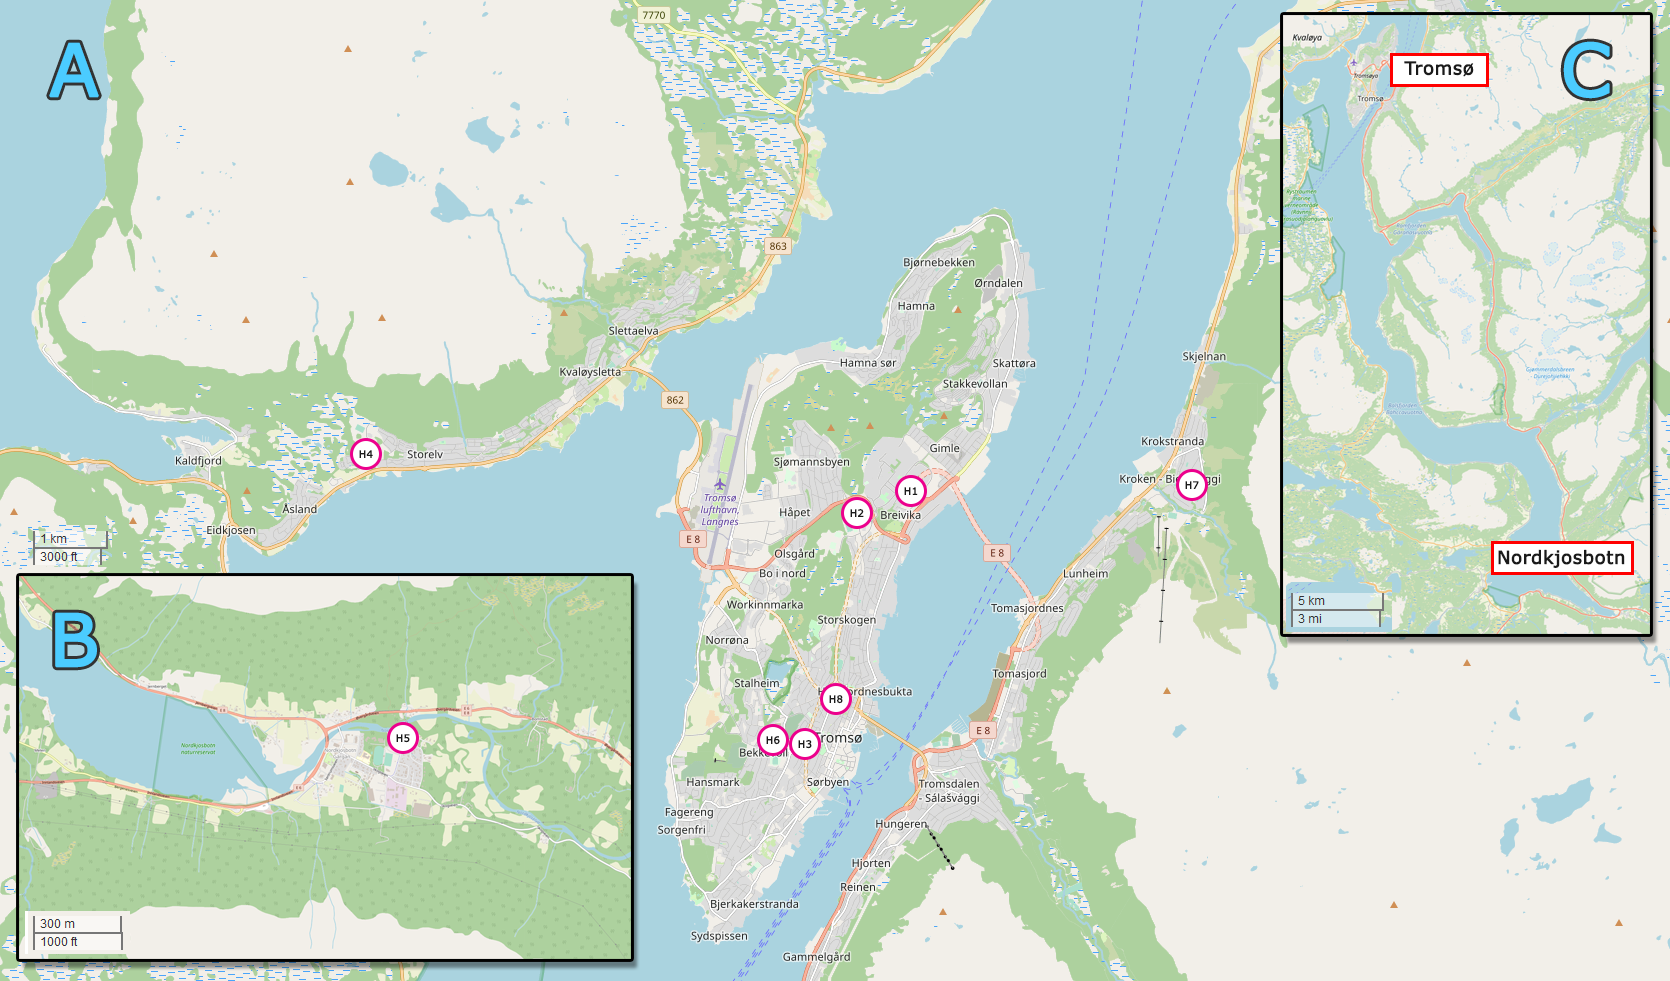
\includegraphics[width=0.9\linewidth]{figures/Methodology/schoolmaps.png } 
        \caption{Geographical location of all eight high schools included in the Fit Futures study. "A" refers to the area around Tromsøya, and "B" is the area in the town of Nordkjosbotn (Balsfjord). "C" shows the distance between "A" and "B".}
        \label{figure:hsLocations}
    \end{figure}

In FF1 and FF2, the participants had a one-day visit to The Clinical Research Unit at the \gls{unn}, which included clinical examinations, microbiological samples, blood samples, a web-based general questionnaire (chapter \ref{ch:Annex}), and an interview \cite{Winther2014}. All procedures were performed by trained research study nurses. 

FF11 and FF12 refer to short follow-ups performed during the FF1 period. In these sub-surveys, not all the data was gathered again; only a sub-sample such as the swabbing of the \textit{S. aureus}.

\subsection{Social network assessment}
\label{method:SocialNetwork}

The social network was constructed based on the following questions in the interview. These were written and answered in Norwegian, here we provide the English translation: \textit{“Which students have you had the most contact with the last week? Name up to 5 students at your own school or other schools in Tromsø and Balsfjord.”}. Reciprocity in the nomination was not mandatory. For each of the nominations, five “yes/no” questions assessed the type of contact they had with their nominations: \textit{“Do you have physical contact?”}, \textit{“Are you together at school?”}, \textit{“Are you together at sports?”}, \textit{“Are you together at home?”}, \textit{“Are you together at other places?”}. This resulted in five social networks: Physical Network, School Network, Sports Network, Home Network, and Other Network. Adding all the relationships together formed a sixth network that was called the Overall Network. Illustrations of all networks are presented in figure \ref{figure:allNetwork}.

Not 100\% of the students participated in the study, and some of the relationship information between them is lost (table \ref{table:SummaryLost}). The final analysis shows that some of the lost 134 IDs, were very popular, with up to 9 friends nominated.

    \begin{figure}[ht!]
        \centering
            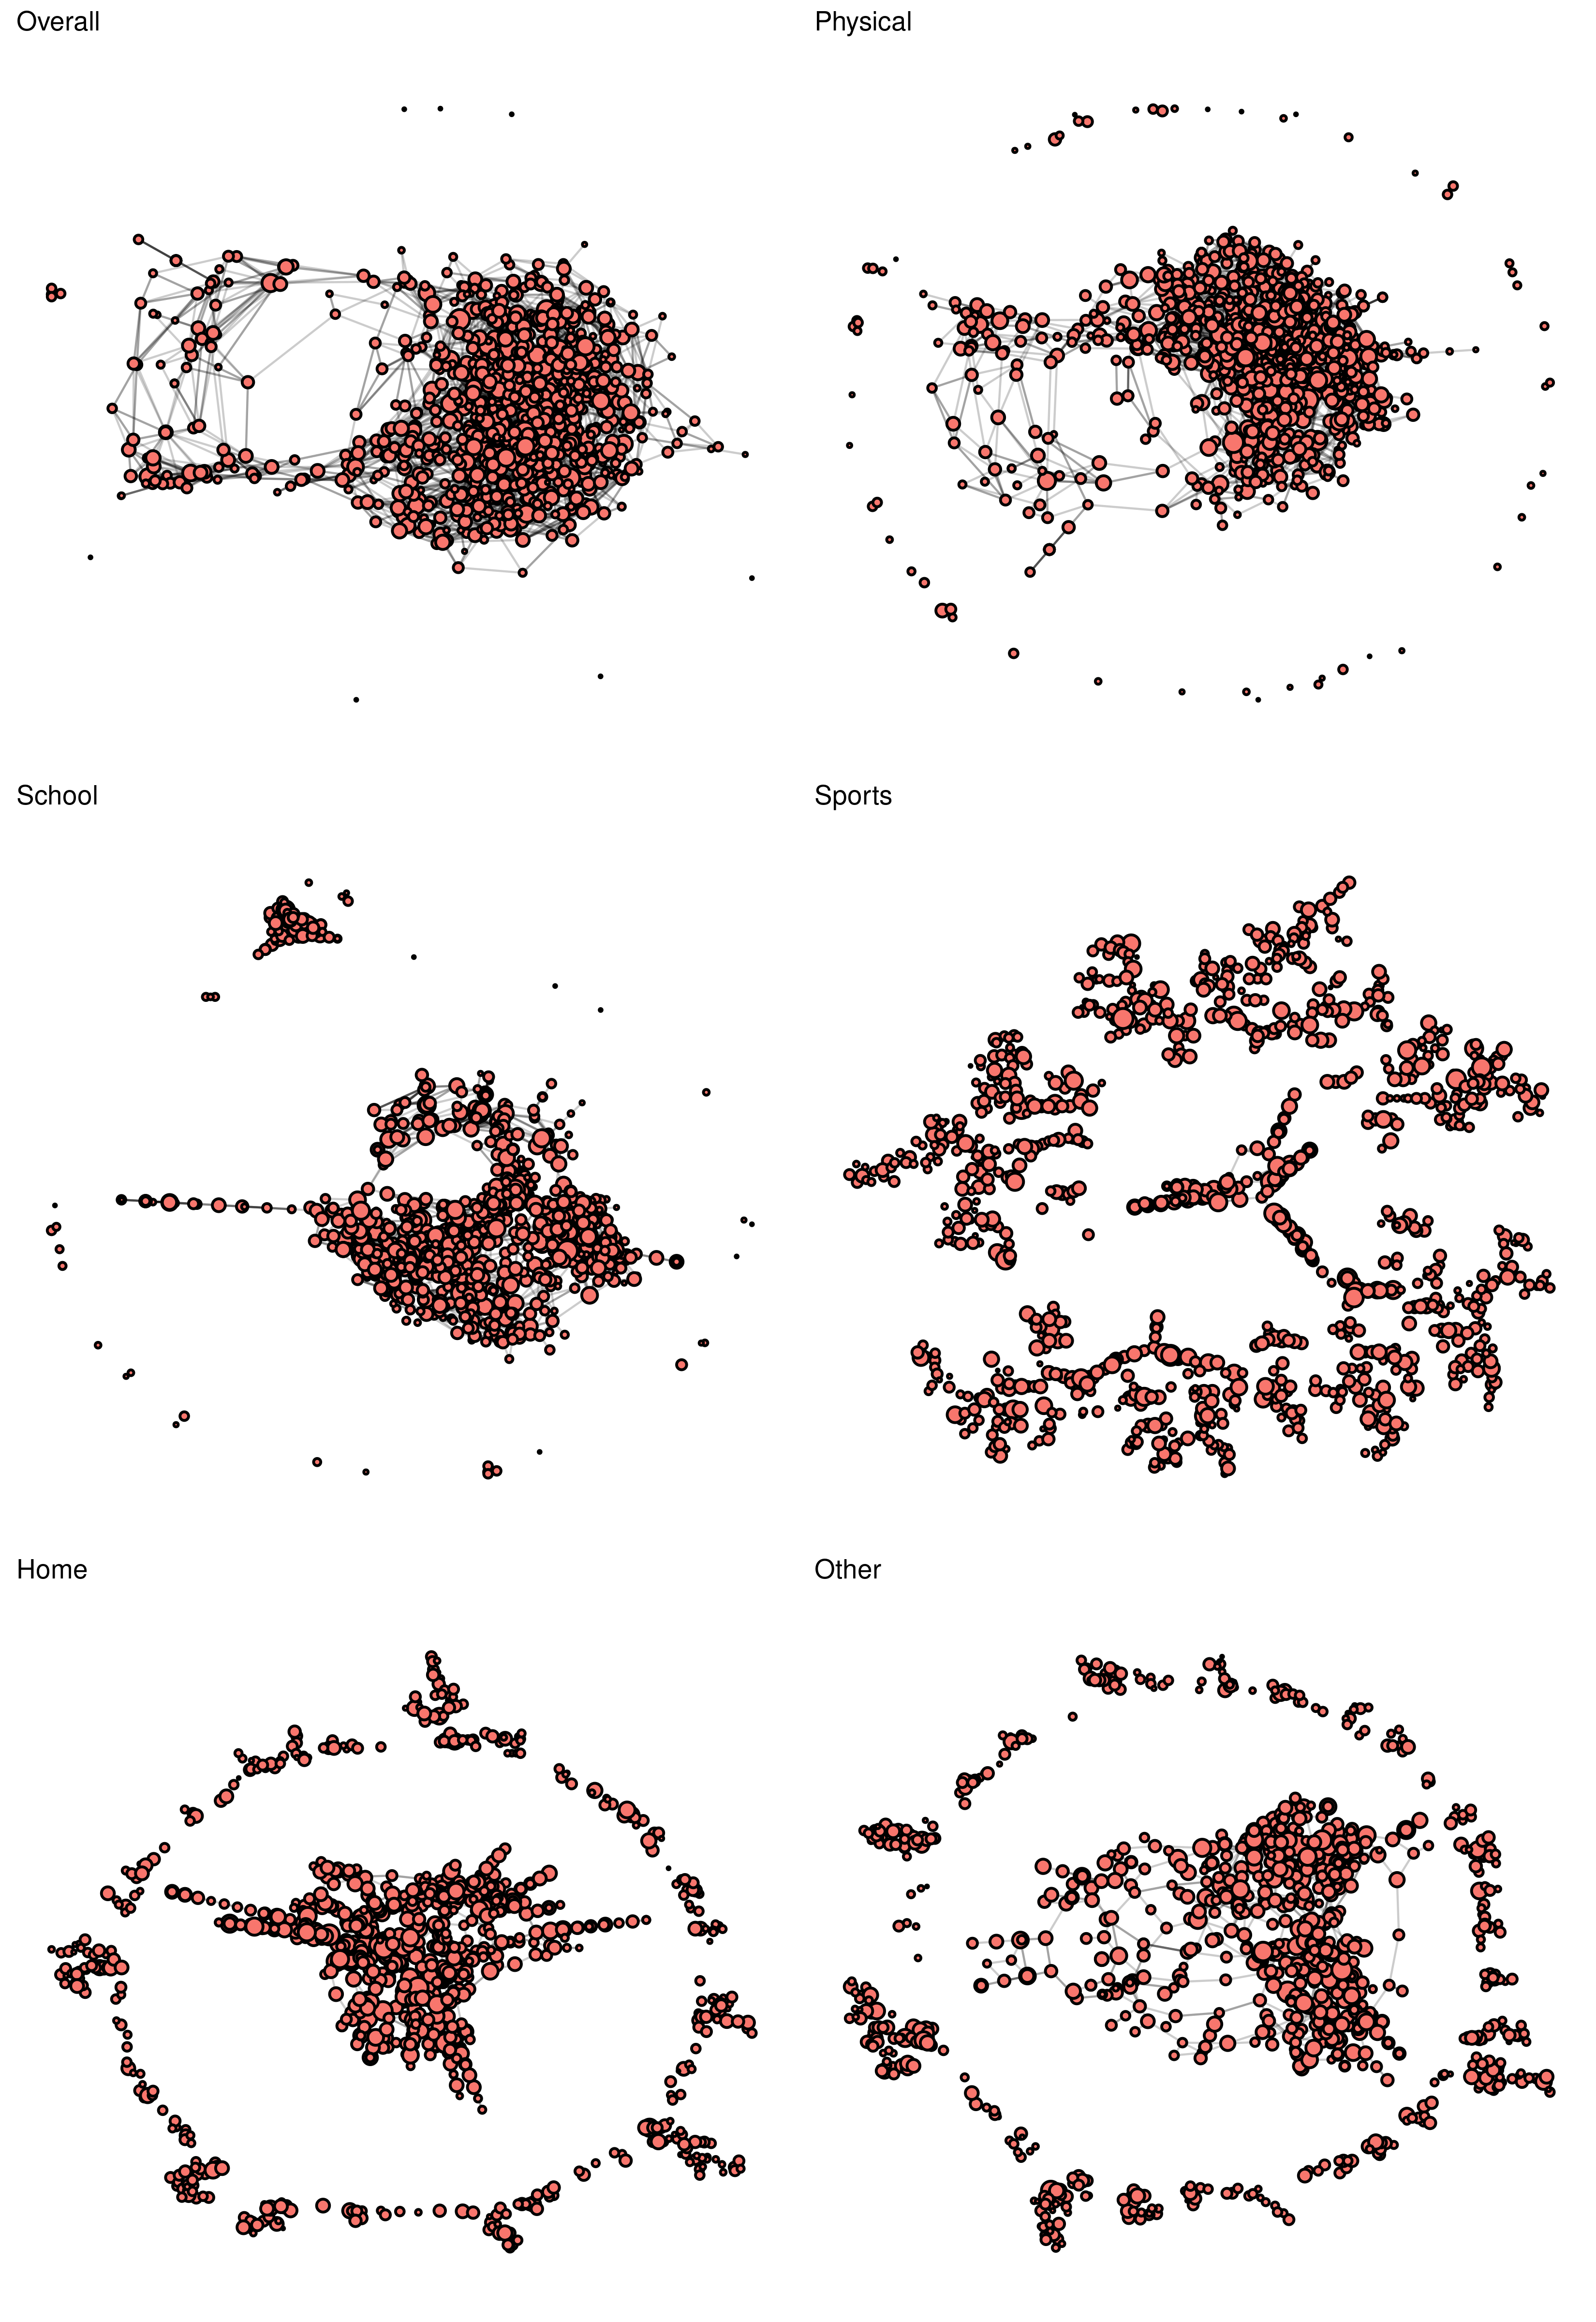
\includegraphics[width=0.8\linewidth]{figures/Methodology/allGraphs.png } 
        \caption{All networks in FF1 following a MDS layout. Each student is represented by one node in the network. Each relationship is represented by an undirected edge, i.e., a line, in the network.}
        \label{figure:allNetwork}
    \end{figure}

    
    \begin{table}[ht!]
    
        \caption{Information with the school names, study program, the total number of students in FF1, astronomical season, and whether a significant amount of students' blood samples were taken during the polar night.}

        \centering

        \label{table:SummarySchools}

        \scalebox{0.75}{
        
        \begin{tabular}{|
        >{\columncolor[HTML]{FFD5D3}}l |lllll|}
        \hline
        \cellcolor[HTML]{FFCCCC}ID           & \cellcolor[HTML]{FFFFC7}Name         & \cellcolor[HTML]{FFFFC7} Studies program &
        \cellcolor[HTML]{FFFFC7}FF1 Students & \cellcolor[HTML]{FFFFC7} Extraction & \cellcolor[HTML]{FFFFC7} Polar night \\ \hline
        
        H1   & Breivika videregående skole     & Vocational             & 207   & Autumn    & No   \\
        H2   & Breivang videregående skole     & Vocational and General & 142   & Autumn    & Yes  \\
        H3   & Kongsbakken videregående skole  & Vocational and General & 168   & Winter    & No   \\
        H4   & Kvaløya videregående skole      & Vocational and General & 98    & Spring    & No   \\
        H5   & Nordkjosbotn videregående skole & Vocational and General & 85    & Spring    & No   \\
        H6   & Norges Toppidrettsgymnas Tromsø & Sports                 & 26    & Spring    & No   \\
        H7   & Tromsdalen videregående skole   & Sports and General     & 192   & Winter    & Yes  \\
        H8   & Tromsø maritime skole           & Vocational             & 120   & Winter    & Yes  \\ \hline
        
        \end{tabular}

        }
    
    \end{table}

To evaluate if the friends mentioned were representative of the participant's social network, the following question was asked: \textit{“To what degree does this table of friends give an overview of your social network? Please indicate on a scale from 0 (small degree) to 10 (high degree).”} Nominated friends that did not participate in FF1 were excluded from the analysis (n=134). In figure \ref{figure:networksRepresentative} we can see a histogram with all the answers.

    \begin{figure}[ht]
        \centering
            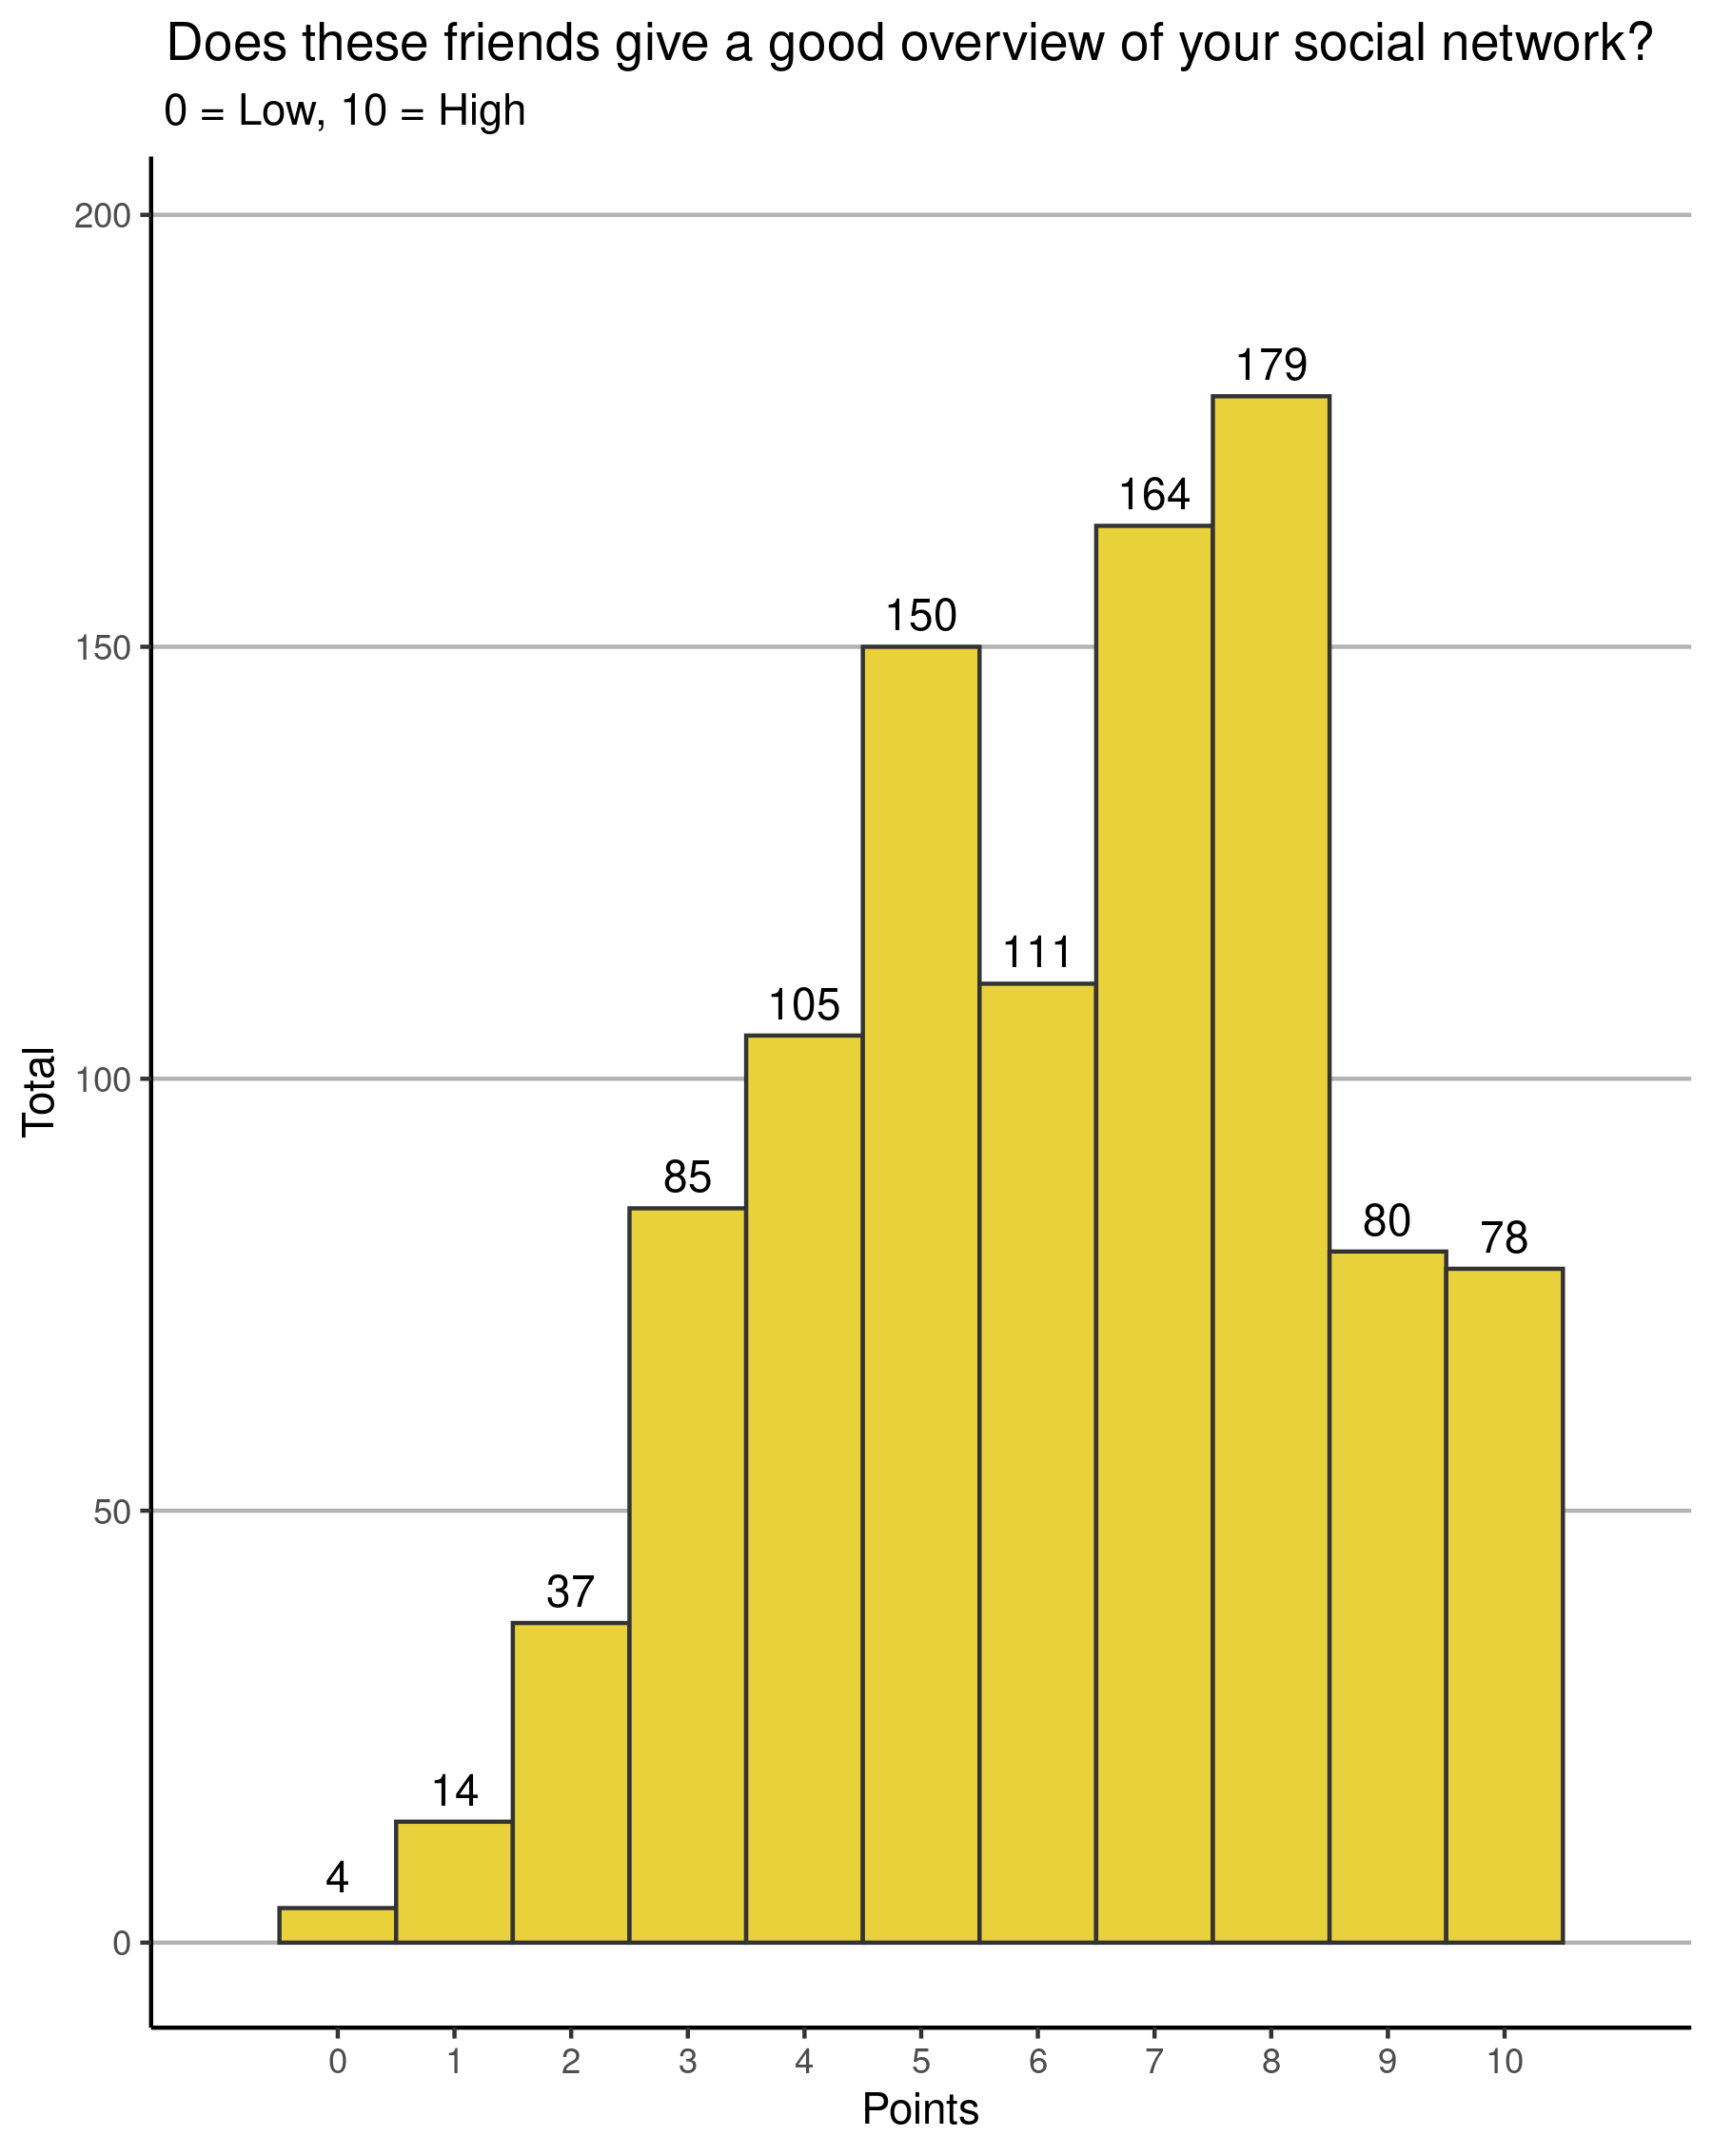
\includegraphics[width=0.55\linewidth]{figures/Methodology/Histogram_completeTable_Overview.png} 
        \caption{Histogram with all the answers to the question: \textit{“To what degree does this table of friends give an overview of your social network? Please indicate on a scale from 0 (small degree) to 10 (high degree).”}}
        \label{figure:networksRepresentative}
    \end{figure}



\begin{table}[ht!]

    \caption{Summary of lost connections at data cleaning.}

    \centering

    \label{table:SummaryLost}

 	\renewcommand{\arraystretch}{1.5} 

    \scalebox{0.75}{
  
    \begin{tabular}{ lll }
        \hline
        \rowcolor[HTML]{FFFFC7}

         \textbf{ Concept } &         \textbf{ Total } &         \textbf{ Relative } \\ 
        \hline 

        \multicolumn{1}{l|}{ Total IDs: } & 1177   & 100 \%          \\ 
        \multicolumn{1}{l|}{ - Total Deleted IDs: } & 139   & 11.81 \%          \\ 
        \multicolumn{1}{l|}{ - Total Remaining IDs: } & 1038   & 88.19 \%          \\ 
        \multicolumn{1}{l|}{ Total Edges: } & 4125   & 100 \%          \\ 
        \multicolumn{1}{l|}{  - Total Deleted Edges: } & 473   & 11.47 \%          \\ 
        \multicolumn{1}{l|}{  - Total Remaining Edges: } & 3652   & 88.53 \%          \\ 

    \end{tabular}
    
    }

\end{table}

\subsection{Host risk factors}

All questions related to sex, use of recreational drugs, dietary habits, chronic diseases, medication usage, sport frequency, sedentism, and so on, are self-reported using a web-based questionnaire.

\subsection{Hormonal contraceptive}

Information on current hormonal contraceptive use was obtained from the interview. \gls{hc} were categorized into combination contraceptives and progestin-only contraceptives. The combination contraceptives were further divided into groups according to high and low ethinylestradiol daily dosage. High dosage was defined as HC containing $\geq$ 30 μg ethinylestradiol. Low dosage was defined as contraceptives containing $\leq$ 30 μg ethinylestradiol. The classification for each brand can be seen in table \ref{table:hormonalDefinitions}.

\begin{table}[ht!]

    \caption{Types of hormonal contraceptives classification and their respective brands.}	

    \centering

    \label{table:hormonalDefinitions}

	\small

	\centering

    \scalebox{0.75}{

	\begin{tabular}{l|l}
	\hline
	\rowcolor[HTML]{FFAAAA} 
	Hormonal type                    & Contraceptive brand  \\ \hline
	Non-hormonal                     & Condoms              \\ \hline
    	                             & Cerazette            \\
        	                         & Nexplanon            \\
            	                     & Depo-provera         \\
	\multirow{-4}{*}{Progestin only} & Implanon             \\ \hline
    	                             & Mercilon             \\
        	                         & Yasminelle           \\
            	                     & Loette 28            \\
	\multirow{-4}{*}{Low Estradiol}  & Nuvaring             \\ \hline
    	                             & Marvelon             \\
        	                         & Yasmin               \\
            	                     & Microgynon           \\
                	                 & Oralcon              \\
                    	             & Diane                \\
                        	         & Synfase              \\
                            	     & Evra                 \\
	\multirow{-8}{*}{High Estradiol} & Zyrona               \\ \hline
	Unknown                           & Any other brand/type
	\end{tabular}
	
    }
	
\end{table}

\clearpage

\subsection{ \textit{S. aureus} assessment}

A first set of nasal and throat swab samples was taken at the research center, and a second set of samples was taken at school after a mean interval of 17 days. All 1038 students were sampled on both occasions, the first batch contained 1028 valid samples, and the second batch 988. A NaCl (0.9\%)-moistened sterile rayon-tipped swab rotated three times with gentle pressure was used to sample both vestibule nasi (nose sample), and an additional swab was used to sample both tonsillar regions (throat sample). The swabs were immediately placed in a transport medium (Amies Copan, Brescia, Italy) and stored at 4°C for a maximum of 3 days. All samples were analyzed at the Department of Microbiology and Infection Control, UNN, both by direct culture \cite{Olsen2011} and enrichment broth (Bacto Staphylococcus medium broth,(Difco Laboratories, Sparks, MD, USA - \cite{Stensen2019}), using blood agar for growth control (Oxoid, UK) and chromID-plates (SAID) for \textit{S. aureus} detection (bioMérieux, Marcy I’Etoile, France). A summary of these methods can be found in the supplementary materials. The growth of any bacterial colonies on agar plates was registered as a valid culture. The most dominating \textit{S. aureus} colony type was frozen at -70°C in glycerol-containing liquid media after confirmation by Staphaurex plus agglutination test (bioMérieux, Marcy I’Etoile, France).



From these results, \textit{S. aureus} nasal or throat persistent carriage was defined as having two \textit{S. aureus} positive cultures for each niche respectively. \cite{Nouwen2004, vanBelkum2009} Two definitions of \textit{S. aureus} persistent carriage was used in the analysis; one based on direct culture, and one based on enrichment broth. All results for every possible combination between the first or second sample, nasal or throat, direct culture or enrichment broth, and so on, can be found in figure \ref{fig:Carrier_definition}. 

%In our context, if a person has \textit{S. aureus} in one sample, we say this person is colonized by the bacteria. If the person has S. aureus in both samples, we say that the person is a persistent carrier. This applies to both the nose and the throat and both the direct culture and enrichment broth. In figure \ref{fig:Carrier_definition} we  encompass all the labeling workflow.

\subsection{SPA typing}

SPA-typing is a technique used to identify the \textit{S. aureus} strain. The gene encoding Spa is highly variable among strains of \textit{S. aureus}, making it a good target for distinguishing different types of bacteria \cite{Hallin2009}. The technique involves targeting the \gls{spa} located in the cell wall are described in the supplementary materials.

For the analysis of \textit{S. aureus} genotype, only data from throat isolates were available (n = 746). All \textit{S. aureus} isolates from throat samples were subjected to spa-typing. The frozen cultures were inoculated on blood agar (Oxoid) and incubated overnight at 37°C. Two or three colonies were transferred to 200 µl sterile\ch{H2O} and vortexed. The isolates were later spa-typed \cite{Sangvik2011}.

\clearpage

            \begin{figure}[!ht]
                \centering
                    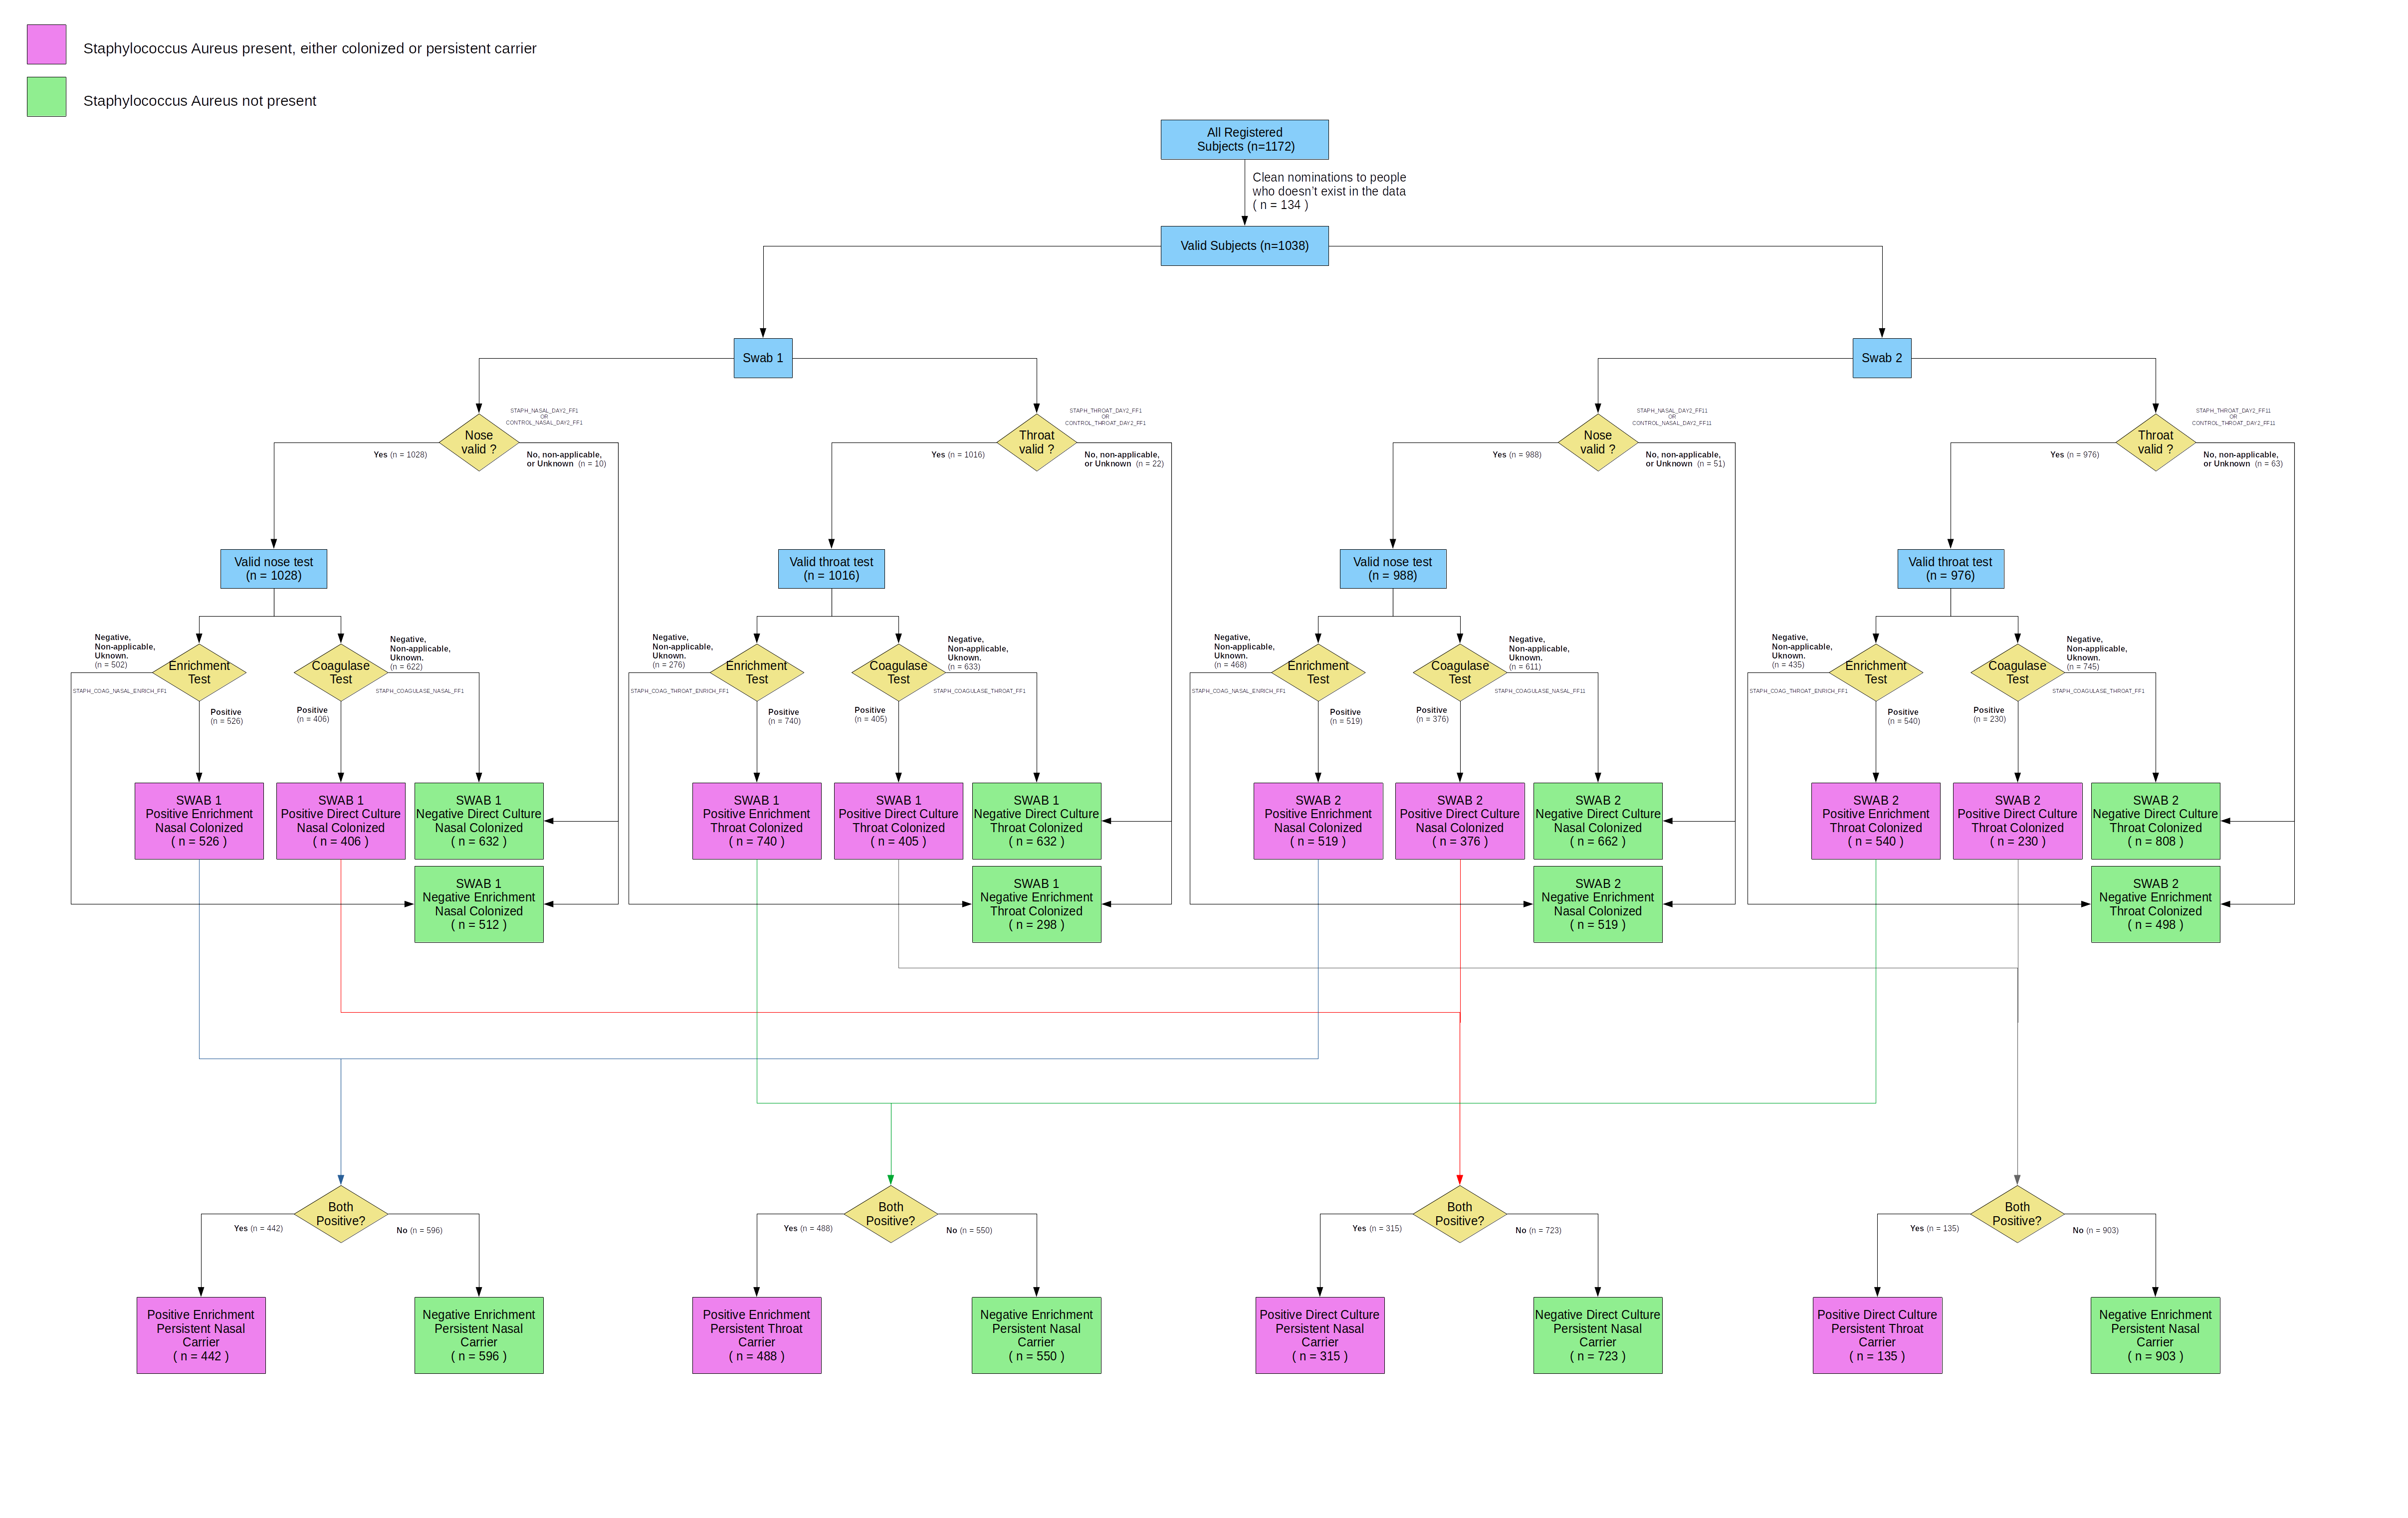
\includegraphics[width=1.2\linewidth, angle=90, origin=c]{figures/Methodology/carrierDefinition.png } 
                \caption{All the S. aureus combinations. A PDF version of this image can be found at the GitHub repository:  \url{https://github.com/rafanozal/PhDThesis/blob/main/Images/carrierDefinition.pdf}}
                
                \label{fig:Carrier_definition}
            \end{figure}

\clearpage

\subsection{Anthropometry assessment}
 
All anthropometric measurements were measured on an electronic scale with participants wearing light clothing and no footwear. BMI is calculated as weight (kg) divided by the squared height ($m^2$) with no correction for sex or age. FF1 has a total of 1034 valid samples, and FF2 has a total of 694.

The BMI comes as a real number and we categorize it following the \gls{who} definition\cite{whoBMI}. "Underweight" if the BMI is lower than 18.5, "Healthy" is above 18.5 and below 25, "Overweight" is between 25 and 30, and "Obese" is greater than 35. The new column is a categorical variable with this information for each person.
  
The WHO also provides BMI-for-age growth charts that take into consideration an individual’s age and sex to determine their BMI percentile. A BMI percentile below the 5th percentile is considered underweight, while a BMI percentile between the 85th and 94th percentiles is considered overweight, and a percentile above the 95th percentile is considered obese. This definition is NOT used since being a relative respects an average rather than a constant value (i.e.: a student being the less obese of a group of people does not make the student not obese); instead, a constant reference point is used as described in the previous paragraph for better comparison across time.

% Describe how does the antropometric variables are measure https://link.springer.com/article/10.1007/s11657-014-0185-0#citeas ; I have no idea why they gave me this reference. Nothing is actually explained there :(

\subsection{Vitamin D assessment}

Blood samples were collected by nurses at the \gls{unn}, centrifugated, and plasma serum was frozen at -70ºC in the Biobank at the \gls{uit}. All samples (n = 890) were sent to the Hormone Laboratory, Haukeland University Hospital, Bergen, Norway; and analyzed by high-pressure liquid chromatography-mass spectroscopy (LC-MS/MS). A sample from all blood vials was reanalyzed at University College Cork, Cork, Ireland, by LC-MS/MS again as a part of the \gls{vdsp} \cite{vdspreference}, and standardization was applied to the rest of the samples \cite{Cashman2015}. 25(OH)D was used as a marker for vitamin D levels. This combines both sources of provitamin D + UVB, and D2+D3 from diet. It has a longer half-life span in blood than other available metabolites. Both 25(OHD)D\textsubscript{2} and 25(OHD)D\textsubscript{3} were measured at the same time. 

\subsection{OLINK Target 96 Inflammation }

Serum levels of 92 proteins were analyzed at the Clinical Biomarkers Facility, SciLifeLab, (Uppsala, Sweden), using the Target 96 Inflammation panel from Olink Holding AB (Uppsala, Sweden) \cite{olinkWeb}. A detailed description of the significance of each marker, alongside the mathematical significance of the values, can be found in the supplementary materials. A total of 936 samples were analyzed this way.

\subsection{Simulations}

\label{sec:MetodologySimulations}


Bootstrapping is a statistical technique used to estimate the variability of a sample statistic without making any assumptions about the underlying population. To determine whether there is bias within the relationships in a network we use bootstrapping simulating 1000 networks using a similar approach to previously described non-parametric tests \cite{ref:nonparametricBook}. This consists of counting how many relationships connect two nodes with the same attributes in our network (i.e., \textit{S. aureus} carrier with \textit{S. aureus} carrier) and comparing this number with the same number given by the simulations. In figure \ref{figure:methodSimulations1} we can see an example of a real network, a simulated one, an arbitrary node attribute distribution, and the same-to-same relationships in each.

    \begin{figure}[H]
        \centering
            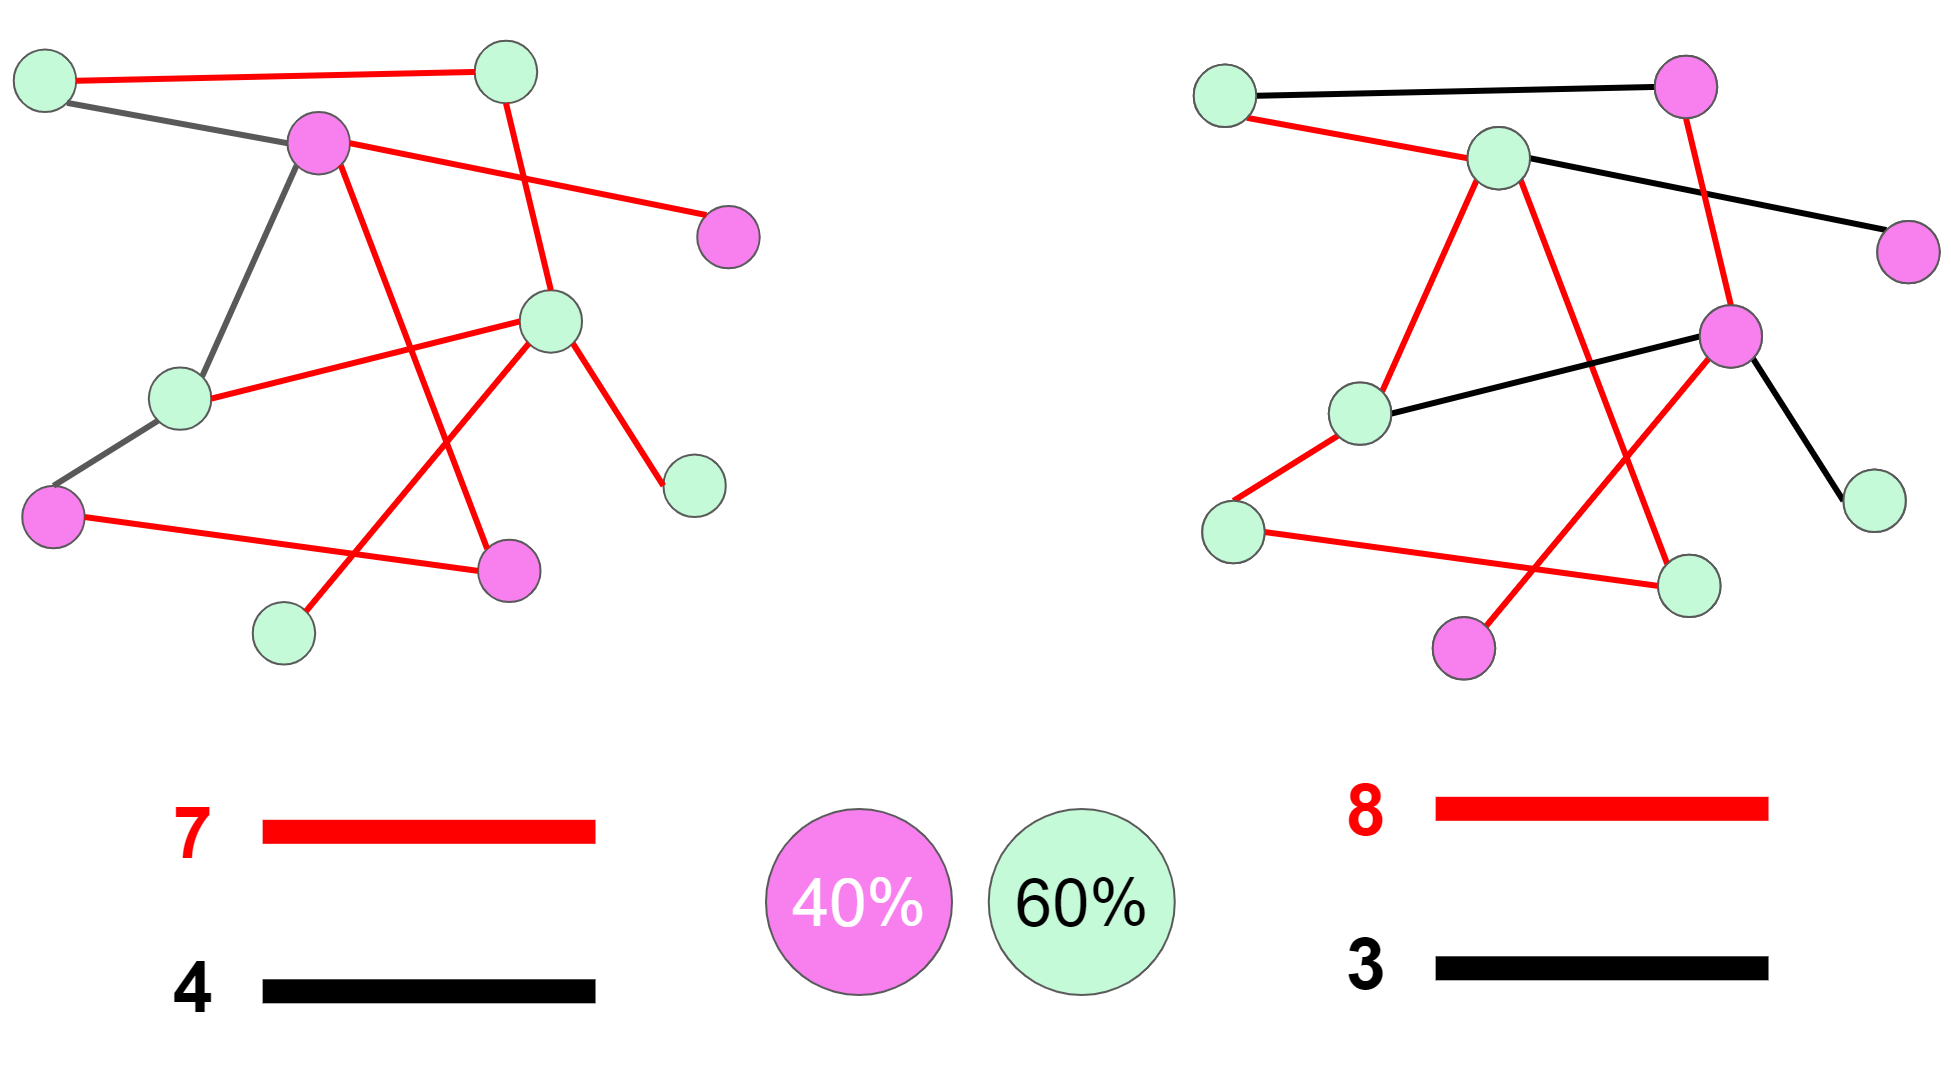
\includegraphics[width=0.7\linewidth]{figures/Methodology/Simulations1.png } 
        \caption{In this figure we see two isomorph networks with the same layout. On the left, we have a representation of a real network. On the right, is a simulated network. Both networks have the same distribution of attributes, with 4 nodes in purple and 6 nodes in green. On the real network, we count 7 edges that share the same node color (same-to-same relationship) which are highlighted in red; while in the simulated network, we count 8. This result indicates that the real network has a bias towards nodes not sharing the same color because the simulation is assumed random and without bias. However, one simulation is not enough, and the result can be due to just random chance. Therefore, the process described on the right is repeated 1000 times, making a distribution of counted same-to-same simulated relationships.}
        \label{figure:methodSimulations1}
    \end{figure}

This gives us a distribution of 1000 values from which we can extract a mean and a standard deviation. We then perform simple hypothesis testing, like a t-test, using the real amount of same-to-same relationships against a normal distribution given by the simulated mean and standard deviation. 

We expand on this concept by instead of using the distribution of attributes in the general population of a node (i.e., \textit{S. aureus} carrier prevalence being 30\%), using the distribution of one specific category (i.e., \textit{S. aureus} carrier prevalence in women being 20\%) and repeating the same process for each category present in each attribute of interest (ie: women and men in sex, from underweight to obese in BMI, and so for). This gives us a new mean which then can be compared with the previous simulated distribution. In this way, we can check how much each of the categories deviates with respect to each other, and we can identify which category has a higher or lower risk for the outcome variable; if any.

Ideally, this technique should be done not by simulating similar networks, but by simulating every possible network and comparing those in which bias happens to those in which bias does not happen. However, it is impossible to find every possible network within reasonable computational time. So we need to reduce the number of possible networks based on some assumptions \cite{Bevan2017}. This allegedly gives the model properties that make it similar enough to all the possible networks. In our case, we use the same frequency tables with a network with the same topology as constriction. We also assume that the virulence of \textit{S. aureus} would cluster carriers with carriers and vice-versa. As BMI homophily is high and the Chi-square table also suggests so, we also assume that this happens with subjects with similar BMI. Finally, we also assume that friends share similar environments and activities and this would be reflected in their vitamin D levels.

\subsection{Friendship ratio}

Biomarkers levels are a continuous variable and as such we cannot use the simulation approach unless we categorize them into something similar to "low level", "medium level", and "high level", losing some information in the process. Instead, we compare numerical levels between friends and non-friends biomarkers one by one. We do this by finding the ratio of, the average square difference between each person's biomarker level and friend's biomarker levels, and the average square difference between each person's biomarker levels and non-friends biomarker levels. Values significantly greater than 1 suggest that clusters of friends have similar biomarker levels in comparison with the rest of the non-friend population, while values smaller than 1 would suggest the opposite. Values similar to 1 suggest nothing, however, we do not know a sensible threshold cut-off for this approach. We arbitrarily suggest that values greater than 1.1 or smaller than 0.9 are the significant ones.

\section{Data cleaning}

\label{datacleaningSection}

%A full report on how the data was transformed, as well as the cleaned data, is available upon request.

This section will present a summary of the important parts of the methodology followed in the data-cleaning process as well as the shortcomings encountered due to the experiment design or the original data-registering process. In the Appendix (chapter \ref{ch:Annex}), some samples from the 25 tables with the original variables' names and a description of what each variable represents are provided, but we do not provide examples from tables that could potentially be used to identify students.

    \begin{figure}[H]
        \centering
            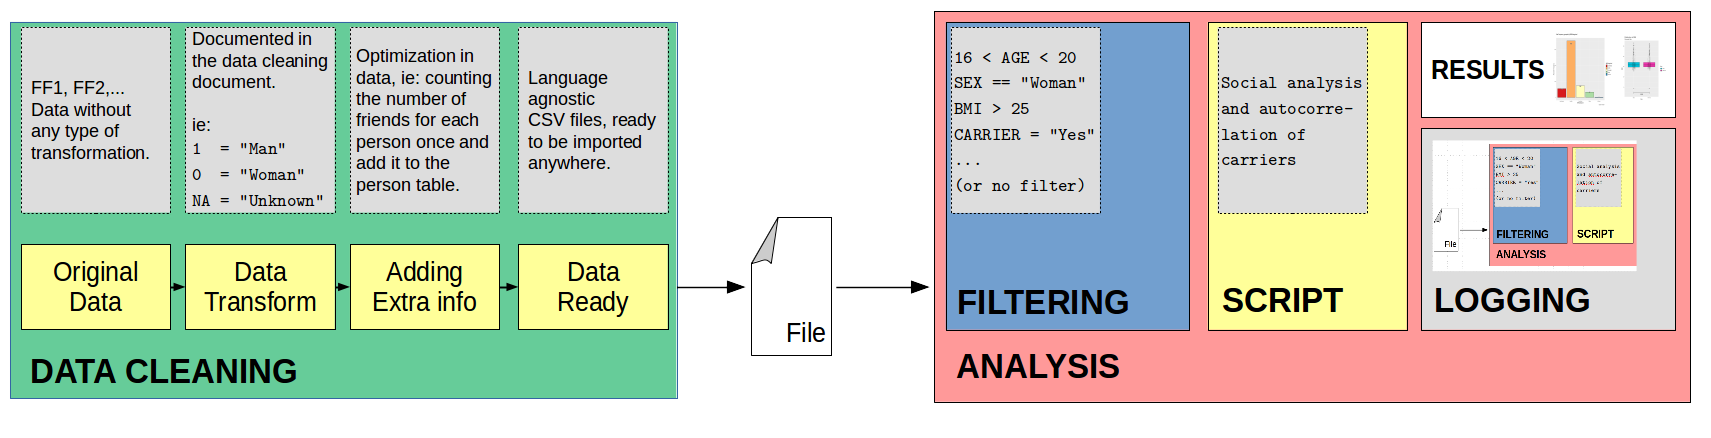
\includegraphics[width=0.95\linewidth]{figures/Methodology/general.png} 
        \caption{Overview of the data cleaning process. To the left, each step that transforms the raw data into a more practical version. This process is done only once. To the right, the subsequent analyses are performed as many times as needed.}
        \label{fig:Data_cleaning_summary}
    \end{figure}

Using our data will save time as it has been thoroughly cleaned, numerical data which is meant to be categorical has been given meaningful strings, diseases with just a verbal description with no code for \gls{icd10} has been assigned manually, and most importantly the data has been transformed into tables following proper Boyce-Codd normalization \cite{ref:KOHLER201888}.


\subsection{Naming}

We changed their name to something more human-friendly and CSV and latex-compatible. This means using upper and lower cases appropriately, "ID" instead of "pers$\_$key$\_$ff1". Samples are labeled as S1 and S2 instead of the given FF11 or FF12 sub-time period. Direct culture and enrichment broth are simplified to "direct" (from STAPH in any case which is confusing) and "enrich". Units are included where possible in the variable name ("FE$\_$FF1" to "Fe$\_$(µmol/L)"). All FF id references are deleted as they are divided into Table$\_$FF1, Table$\_$FF2, and so on. Adding variable name continuity to quickly discern between binary and categorical variables ("FAT$\_$FISH$\_$FF1" to "FatFishFrequency") so the user already knows what to expect in each column. Deleting redundancy in names (  "FRIEND2$\_$CONTACT$\_$SCHOOL$\_$FF1" to "Friend2School").

\subsection{Dates}

For all tables where a date appears, dates are standardized from several data formats (Posix, "mm/dd/YY", "dd/mm/YY", "YYYY-MM-DD") to "YYYY-MM-DD" format. Some of the dates could be transformed to have more precision down to "HH:mm:ss" resolution, but this information is irrelevant to us anyway so it is discarded. SPSS is the programming language that is used to encode the original data, and it uses the start of the Gregorian Calendar in 1582 as the default date for POSIX origin. Because of this chosen date reference, there might be some days' error in coercion in these dates because we do not know which timezone, or time origin, we take as a reference. We delete all timezones from UTC to simply a date, which we assume is GMT +1/+2 depending on the time of the year. Since the time difference is one to two hours, and we have a day resolution level, this loss of detail does not matter. It is advisable to use another non-SPSS method in the future as this time error coercion might render biological data which is time-critical unusable.

\subsection{General tables}

\subsubsection{\textit{S.aureus}}

These tables contain the \textit{S.aureus} information. Note that none of the FF11 variables are described in the metadata files. The information was retrieved from Fit Future experiment designers.

\subsubsection{Swabbing information}

All lab comments that are just registered as \textit{"OK"} by lab technicians for all samples are discarded to avoid data redundancy. Also, all status and event variables are redundant information and are later discarded. All leading and trailing white spaces are deleted. None of these variables are described in the metadata and information.

What remains, for each unique nasal and throat swab, is whether the swabbing was performed successfully, with irregularities and the given reason, the swab was repeated, or the swab was not performed at all. We also have the freezer ID of where to find each sample as well as the freezing date.

\subsubsection{Blood serum and Blood Technical information}

Several variables indicate if some value is above or below the healthy limit which are discarded. The reference on whether some value is healthy or not is marked during the analysis according to the given references for each value. Within the blood serum scope, there are also a bunch of columns named EVENT0 to EVENT9, and EVENTA to EVENTL, which are empty, no description is given in the metadata or any other source, and have no information at all. As such all of them are deleted. All LCMSMS (Mass spectrometry measures) have the same values as their normal measurements counterparts, so those are also skipped.

\subsection{Relational Normalization}
\label{ssec:normalization}

The original data does not have any type of relational meaning between columns. To add future benefits, we need to fix this issue due to privacy security \cite{DomingoFerrer2009}, data logical consistency \cite{DomingoFerrer2009}, and computational time efficiency. This section describes all tables related to relational data. The medicine, contraceptive, and disease tables are read from the original dataset and then transformed later into a structure that follows a proper relational database property.

%\subsection{Formatting}

%In the previous section, we have described which type of data is available to us. Here we are going to explain how the data is clean and transformed into something more useful. The process consists of importing the data from the files described previously with no type of filter. Then transform the original data into values that are more meaningful, as well as add new columns to our data based on data that we already have (i.e.: whether a person is \textit{S. aureus} carrier or not). Then prepossessing the data and adding columns that are time intensive (i.e.: searching for all the friends for all the people, and counting how many types of relationships they have, takes a lot of computational time when you have to do it thousands of times, but you don't need to do this every time you run the network analysis). Finally, we need to normalize the diseases and medicine tables into a proper relational structure. Same for the contraceptive table which is a special case of the medicine table.

%After all of these steps, the data is finally clean and ready to use. But we don't use the data just yet. We save this final version into CSV files and later on we apply the filtering variables with whatever restrictions you want (i.e.: age from 15 to 18). This way, the data cleaning, filtering, and analysis are independent of each other. Notice that data stratification happens where needed during the analysis (i.e.: table for women and table for men); this operation is always O(n) and doesn't need a lot of time to be carried on as it doesn't need to transform all the graphs regarding friendship again and again.


%In all cases, first, we are going to change the selected variable names to something more meaningful; the same for the categorical values that are encoded as numbers.

%\subsubsection{Naming}

%All the variables that we named in the previous chapter changed their name for something more human-friendly and CSV and latex-compatible. This means using upper and lower cases appropriately, "ID" instead of "pers$\_$key$\_$ff1". Samples are labeled as S1 and S2 instead of the given FF11 or FF12 sub-time period. Direct culture and enrichment broth are simplified to "direct" (from STAPH in any case which is confusing) and "enrich". Units are included where possible in the variable name ("FE$\_$FF1" to "Fe$\_$(µmol/L)"). All FFX references are deleted as they are divided into Table$\_$FF1, Table$\_$FF2, and so on; since are implicitly declared at the table level the extra characters are redundant at the variable level. Adding variable name continuity to quickly discern between binary and categorical variables ("FAT$\_$FISH$\_$FF1" to "FatFishFrequency") so you already know what to expect in each column. Deleting redundancy in names (  "FRIEND2$\_$CONTACT$\_$SCHOOL$\_$FF1" to "Friend2School").

\label{relationalNormalization}
%\subsubsection{Relational Normalization}

The data should be organized in Boyce–Codd normal form \cite{ref:KOHLER201888}. Boyce-Codd normalization is important because it ensures that there are no data dependencies between columns, which translates into guaranteeing the integrity and consistency of data which is critical for accurate analysis. This is also crucial in datasets with large amounts of data, but this is not the case. Summarizing the normalization process, all variables and data in those tables need to be transformed so they follow these fundamental principles of normalization:

\begin{itemize}

    \item \textbf{0NF} No information is lost and no information is duplicated.
    \item \textbf{1NF} No columns, or multicolumns (3NF), which contain sets of values.
    \item \textbf{2NF} Single column primary key (person ID) which is also used as superkey (4NF).
    \item \textbf{3NF} Eliminating the transitive functional dependencies.
    \item \textbf{BCNF} Always satisfies lossless join condition.

\end{itemize}

\begin{figure}[H]
        \centering
            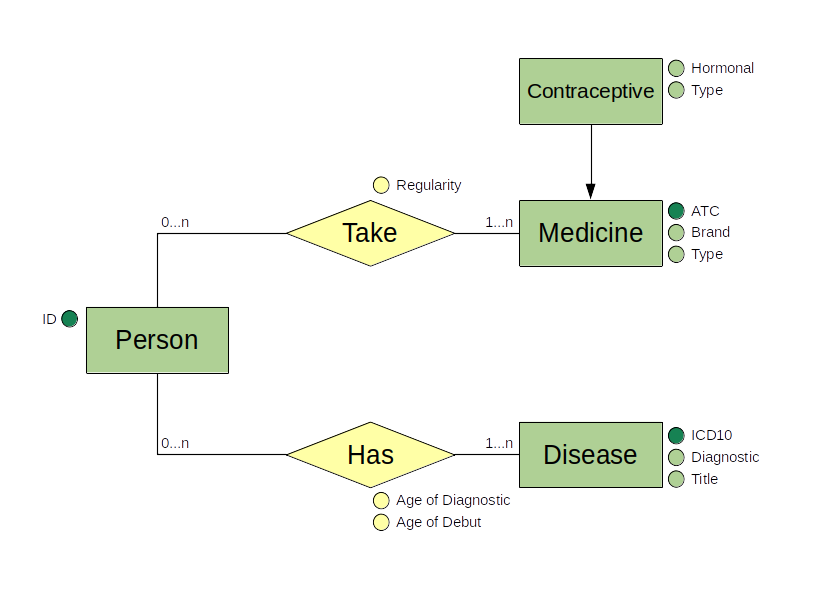
\includegraphics[width=0.75\linewidth]{figures/Methodology/DBrelationals.png} 
        \caption{BCNF transformation from the original data. The database schema for "Person" can be obtained upon request.}
        \label{fig:Database_relational_image}
\end{figure}

%Further information about what compromises the "person" table can be found in the appendix, in section \ref{chapter:Annex_schema}.

%In other tables, similar transformations are produced. Which we will see one by one in the next section. However, because this dataset is not especially big, we applied the join operations to all tables and saved the result in our files. This actually fails the non-duplicity condition and increase significantly the CSV file size, but we do it anyway to increase performance in R (which otherwise would be quite slow having to do joining operations over and over). The disjoint operation is quite trivial if needed (just unique by ID and ICD10, and ID and ATC). The final results for the diseases, medicine, and contraceptive tables, are as follows:

%\begin{table}[H]

	%\tiny	

    %\centering

    %\label{table:Diseases_DB}
    
	%\renewcommand{\arraystretch}{1.5}

    %\begin{tabular}{| l | p{10cm}  l }
     %   \hline
      %  \rowcolor[HTML]{FFAAAA}

       % \textbf{Name} & \textbf{Description} \\ 
        %\hline 

        %\multicolumn{1}{l|}{\detokenize{ID}}             & Person ID \\ 
        %\multicolumn{1}{l|}{\detokenize{Diagnostic}}     & Name of the disease \\ 
        %\multicolumn{1}{l|}{\detokenize{ICD10}}          & Disease identifier following ICD10 \\ 
	    %\multicolumn{1}{l|}{\detokenize{Title}}          & Group to which the disease belongs ("Skin and subcutaneous tissue", "Respiratory system"...) \\
        %\multicolumn{1}{l|}{\detokenize{Age_Diagnostic}} & At what age where you diagnose for the first time \\ 
        %\multicolumn{1}{l|}{\detokenize{Age_Debut}}      & At that age where the symptoms first appeared \\ 

    %\end{tabular}%

    %\caption{Table with the final disease variables in relational format.}
    
%\end{table}

%\begin{table}[H]

	%\tiny	

    %\centering

    %\label{table:Medicine_DB}
    
	%\renewcommand{\arraystretch}{1.5}

    %\begin{tabular}{| l | p{10cm}  l }
     %   \hline
      %  \rowcolor[HTML]{FFAAAA}

       % \textbf{Name} & \textbf{Description} \\ 
        %\hline 

        %\multicolumn{1}{l|}{\detokenize{ID}}         & Person ID \\ 
        %\multicolumn{1}{l|}{\detokenize{Type}}       & Group of the medicine ("Antiinfectives for systemic use", "Genito-urinary system and sex hormones")\\ 
        %\multicolumn{1}{l|}{\detokenize{Brand}}      & Name of the medicine ("Ery-Max", "Microgynon", "Paracetamol", "Ibux 400 mg") \\ 
	    %\multicolumn{1}{l|}{\detokenize{ATC}}        & Medicine ID following the ATC codes.\\
        %\multicolumn{1}{l|}{\detokenize{Regularity}} & How often do you use it \\ 

    %\end{tabular}%

    %\caption{Table with the final medicine variables in relational format.}
    
%\end{table}

%\begin{table}[H]

	%\tiny	

    %\centering

    %\label{table:Contraceptives_DB}
    
	%\renewcommand{\arraystretch}{1.5}

    %\begin{tabular}{| l | p{10cm}  l }
     %   \hline
      %  \rowcolor[HTML]{FFAAAA}

       % \textbf{Name} & \textbf{Description} \\ 
        %\hline 

        %\multicolumn{1}{l|}{\detokenize{ID}}         & Person ID \\ 
        %\multicolumn{1}{l|}{\detokenize{Brand}}      & Name of the medicine ("Microgynon", "Cerazette") \\ 
	    %\multicolumn{1}{l|}{\detokenize{ATC}}        & Medicine ID following the ATC codes.\\
        %\multicolumn{1}{l|}{\detokenize{Type}}       & Contraceptive type ("Subdermal", "Oral", "Condoms")\\
        %\multicolumn{1}{l|}{\detokenize{Hormonal}}   & Type of hormone used ("Non-hormonal", "Progestin", "Low Estradiol" )\\ 

    %\end{tabular}%

    %\caption{Table with the final contraceptives table in relational format.}
    
%\end{table}

%There is further transformation to individual data cells in these tables that has nothing to do with the normalization process (ie: translating from Norwegian or standardizing disease names), or defining which type of hormonal contraceptive each brand medicament belongs to.

\subsection{IDs transformation}

Each individual has a personal key described in the \detokenize{"pers_key_ff1"} variable. The original key looks like this: "12345678" and is simply an 8-digit unique key for each of the 1038 individuals in that file. To avoid visual cluttering and math optimization, we substitute the original IDs with an integer number that goes from 1 to 1038, assigned randomly to each individual.

We have two special IDs. An ID equal to 0 means that a person has a friend that is not in our ID table, for example, it could be a student in another school that is not in Tromsø, or Balsfjord; in short, people who were not part of this study. An ID equal to -1 means no friend. This ID numbering keeps consistency later on when we do the filtering. This way, all the variables for each of the 5 friends have an integer, and is easier and faster to do math, indexing, and filtering. ID swapping log is registered in case identifying the original person is necessary but kept confidential.

%In this process of deleting people who are "unknown", we also delete friendship nominations from people who are registered towards people who are unknown. We don't know how many nominations are from people who are unknown to people who exist because we haven't asked those people who are their friends, so the original number of nominations and how many we lost is impossible to calculate. We can tell however how many nominations we have between people who are registered, plus the nomination from registered to unknown (with unknown to registered missing)

%This is the summary of nodes and edges lost in this process:


%\begin{table}[H]
 %   \centering

  %  \resizebox {0.5\textwidth}{0.1\textheight}{ 

% 	\renewcommand{\arraystretch}{1.5} 
 %   \begin{tabular}{ lll }
  %      \hline
   %     \rowcolor[HTML]{FFFFC7}

    %     \textbf{ Concept } &         \textbf{ Total } &         \textbf{ Relative } \\ 
     %   \hline 

      %  \multicolumn{1}{l|}{ Total IDs: } & 1177   & 100 \%          \\ 
       % \multicolumn{1}{l|}{ - Total Deleted IDs: } & 139   & 11.81 \%          \\ 
        %\multicolumn{1}{l|}{ - Total Remaining IDs: } & 1038   & 88.19 \%          \\ 
%        \multicolumn{1}{l|}{ Total Edges: } & 4125   & 100 \%          \\ 
 %       \multicolumn{1}{l|}{  - Total Deleted Edges: } & 473   & 11.47 \%          \\ 
  %      \multicolumn{1}{l|}{  - Total Remaining Edges: } & 3652   & 88.53 \%          \\ 

    %\end{tabular}
 %} 
 
    %\caption{Summary of lost connections at data cleaning.}
    %\label{table:SummaryLost}

%\end{table}

%\begin{figure}[H]
 %       \centering
  %          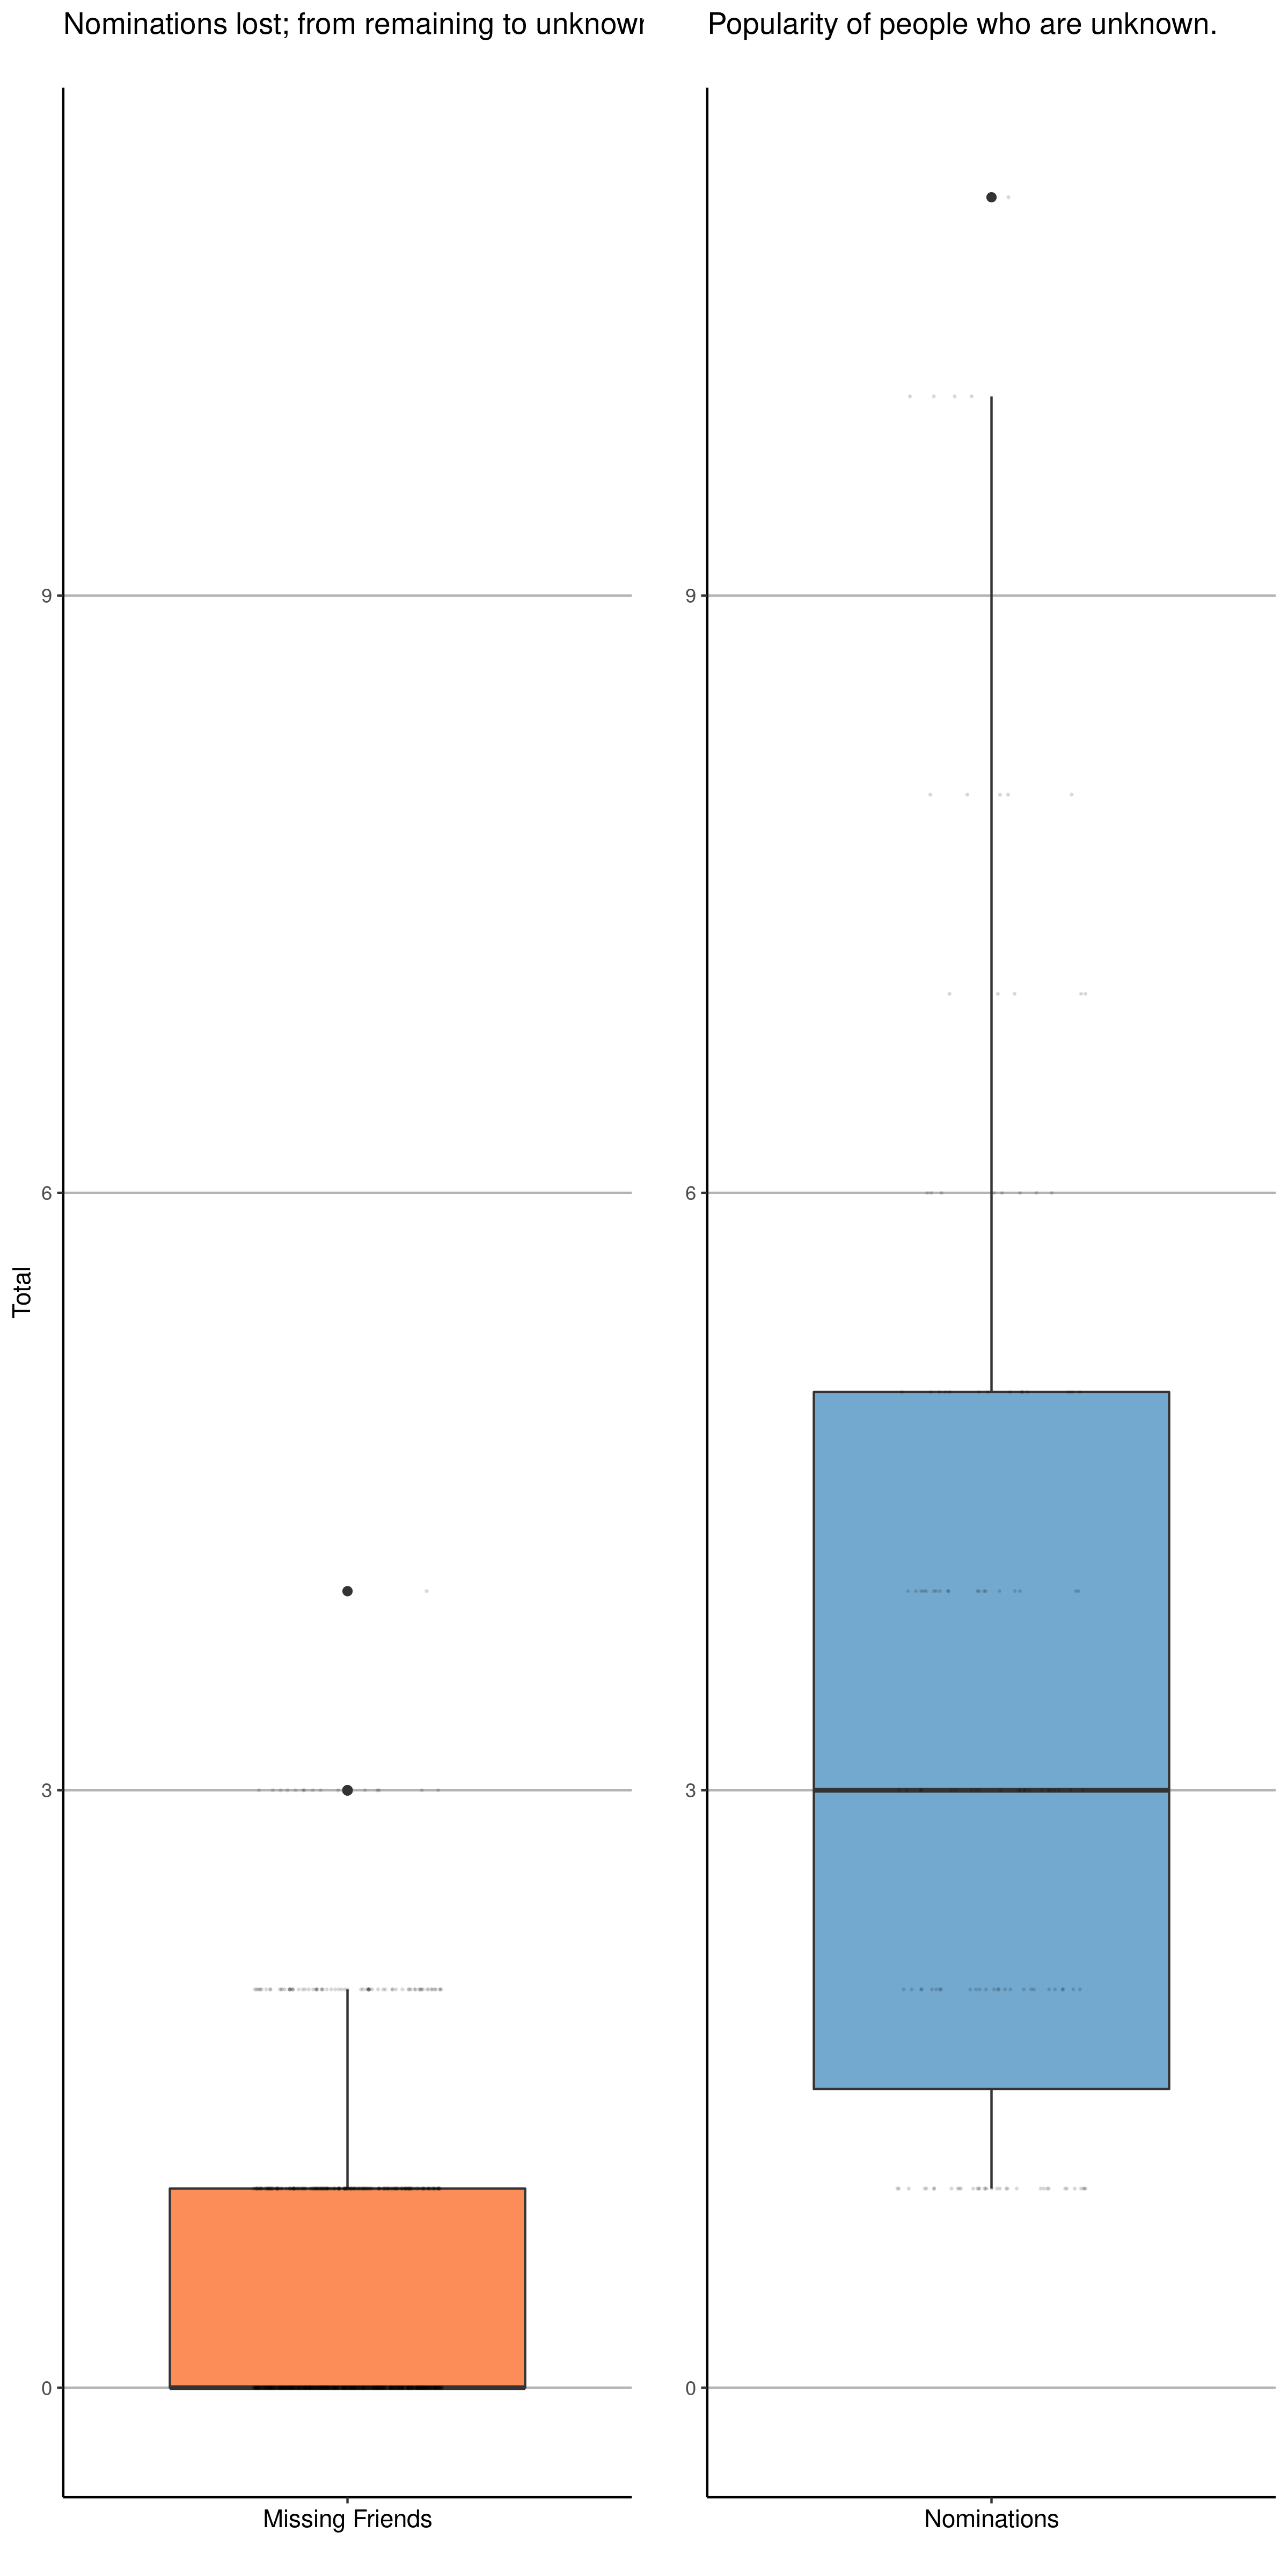
\includegraphics[width=0.2\linewidth]{figures/Methodology/NominationsBoxplots.png} 
   %     \caption{Summary of all nominations lost}
    %    \label{fig:boxplotLostNominations}
%\end{figure}

\subsection{Mapping}

In this subsection, we discuss the relevant issues that arise during the mapping and transformation of the original variables. From the subsequent 29 tables generated during the mapping, we only provide a few relevant examples in this thesis.

\subsubsection{\textit{S. aureus}}

Changes for Nasal and Throat variables are identical. This is also true for the variables for sample 1 and the variables for sample 2. In total, we have Nasal Sample 1, Nasal Sample 2, Throat Sample 1, and Throat Sample 2. Notice that all SPA-type variables remain the same.

\subsubsection{School and education}

Three columns represent "HighSchool", "Class", and "Programme". All of those have a numerical ID to represent the high school, a numerical ID to represent each class, and so on. While those can work ok the way they are, I choose to change them by adding a letter to each column to categorize it properly; these are not numerical values, these are categories. So high-school "1" becomes "H1", high-school "2" becomes "H2", class "10" becomes "C10", program "23" becomes "P23", and so for all values.

\subsubsection{Sociology}

Two variables expressed if "You live with 1 to 2 Siblings (yes/no/NA)", and "You live with 3 or more siblings (yes/no/NA)". Ideally, the questions should be: "How many siblings do you have? (number)", "How many siblings live with you? (number)". But we do not have that. However, we can convert those two variables into a single categorical variable that is expressed as "How many siblings live with you? (NA / Zero / One or Two / Three or more)". Regarding working status, the original data is also divided into too many variables that should not be, as they are sometimes mutually exclusive. The first one is "Is your mother studying?", "Is your mother a housewife?", and "Is your mother disabled?". All three of those are okay to have them separated as any combination of those (yes/no), plus working status, is possible. The rest of the possible answers refer to "Full time", "Part-time", "Unemployed", "Pensioned", "Deceased", "Don't Know", and "Other". All of those are grouped into the same variable within the same variable. Regarding ethnicity, the original question is not clear, and people have not answered ethnicity directly; instead, they have a combination of their country of origin, country of residence, country of parents, and their own race or cultural background. So here is the attempt to clear all that data into something useful. The final variable is a string with as many ethnicities as needed ("Norwegian", "Norwegian-Sami", "Belgium-Spain-France"). People who said they are Norwegian, Sami, or Kven, have a combined ethnicity if answered more than one of those, and also combined with whatever they write in the "Other" column where applicable.

We must express our concern that sharing the precise text from the "Other" category may lead to the identification of individuals. Researchers seeking access to the FF data can, however, apply for access to obtain the exact methodology. 

%People who already answered "Norwegian", "Sami", or "Kvensk" and not included in the "Other" translation if they also include one of those three in the "Other" field. People who emphasize they are from North Norway keep their Norwegian ethnicity (3). People who write "fjellfin" are set to "Sami" instead (2). People who are joking or write some invalid text do not get any follow-up ethnicity (1).

Finally, we have these variables which are just a straightforward mapping \textit{"Who do you live with? / What is your parents' educational background?"} In this case, while would be a fringe case, is possible to live with multiple combinations of these at the same time. For example, parents can be divorced while the student lives with both of them half of the time, each having a stepmother/stepfather, while the grandfather also lives inside one of the houses. So all of these variables are kept independent.


\subsubsection{Puberty and Sleeping}

These tables and serve as an example in which categorical data is overdone due to the string field limitations of SPSS/STATA data. 

The variable for "At what age did your pubic hair start growing?" is, originally, saved as a categorical variable, that gets the values "1", "2", "3", "4", "5", "6", "7", that means from 9 to 15 years accordingly. This is changed from a categorical to a numerical value, however, the data is of course censored to the left and to the right since we do not have any other option. Ideally, we should have a real number instead of the category. For the rest of the men variables we have standardized all answers and eliminated references to the variable in each of the options, so instead of "Facial hair has not yet started growing", or "Voice has not yet started changing", both are mapped to "Haven't Started".

In table \ref{table:Table_Sleeping_Mapping} we see that modeling a time of the day, into 18 different categories is not practical. A better solution would be, at the questionnaire level, to ask "At what time do you go to sleep?" so we can have a numerical value instead. This particular mapping is later transformed into "How many minutes since noon passes until sleeping time", which is a more sensible data format.

\begin{table}[H]

    \caption{Original values for the sleeping habits.}

	\tiny

	\centering

    \label{table:Table_Sleeping_Mapping}
    
	\renewcommand{\arraystretch}{1.5}

    \begin{tabular}{l | l | l}
		\hline
        \rowcolor[HTML]{FF9999}		
		
        \textbf{Variable} & \textbf{Original} & \textbf{Transformed} \\ 		
        
        \hline 
                                  
            \multirow{5}{*}{SleepingPills}
                            
            	& \multicolumn{1}{l}{1}     & \multicolumn{1}{l}{Not used}                 \\\cline{2-3}
                & \multicolumn{1}{l}{2}     & \multicolumn{1}{l}{Less frequently than every week}   \\\cline{2-3}
				& \multicolumn{1}{l}{3}     & \multicolumn{1}{l}{Every week, but not daily} \\\cline{2-3}
				& \multicolumn{1}{l}{4}     & \multicolumn{1}{l}{Daily}   \\\cline{2-3}
				& \multicolumn{1}{l}{NA}    & \multicolumn{1}{l}{Didn't Answered}              \\\hline                                                                                                
   
            \multirow{18}{*}{BedTimeHourCat}
                            
            	& \multicolumn{1}{l}{1}     & \multicolumn{1}{l}{18:00 or earlier}                 \\\cline{2-3}
                & \multicolumn{1}{l}{2}     & \multicolumn{1}{l}{18:30}   \\\cline{2-3}
				& \multicolumn{1}{l}{3}     & \multicolumn{1}{l}{19:00} \\\cline{2-3}
				& \multicolumn{1}{l}{4}     & \multicolumn{1}{l}{19:30}   \\\cline{2-3}
            	& \multicolumn{1}{l}{5}     & \multicolumn{1}{l}{20:00}                 \\\cline{2-3}
                & \multicolumn{1}{l}{6}     & \multicolumn{1}{l}{20:30}   \\\cline{2-3}
				& \multicolumn{1}{l}{7}     & \multicolumn{1}{l}{21:00} \\\cline{2-3}
				& \multicolumn{1}{l}{8}     & \multicolumn{1}{l}{21:30}   \\\cline{2-3}
            	& \multicolumn{1}{l}{9}     & \multicolumn{1}{l}{22:00}                 \\\cline{2-3}
                & \multicolumn{1}{l}{10}    & \multicolumn{1}{l}{22:30}   \\\cline{2-3}
				& \multicolumn{1}{l}{11}    & \multicolumn{1}{l}{23:00} \\\cline{2-3}
				& \multicolumn{1}{l}{12}    & \multicolumn{1}{l}{23:30}   \\\cline{2-3}
            	& \multicolumn{1}{l}{13}    & \multicolumn{1}{l}{00:00}                 \\\cline{2-3}
                & \multicolumn{1}{l}{14}    & \multicolumn{1}{l}{00:30}   \\\cline{2-3}
				& \multicolumn{1}{l}{15}    & \multicolumn{1}{l}{01:00} \\\cline{2-3}
				& \multicolumn{1}{l}{16}    & \multicolumn{1}{l}{01:30}   \\\cline{2-3}															& \multicolumn{1}{l}{17}    & \multicolumn{1}{l}{02:00 or later}   \\\cline{2-3}								
				& \multicolumn{1}{l}{NA}    & \multicolumn{1}{l}{Didn't Answered}              \\\hline                                                                                                

        \end{tabular}

    

\end{table}

\subsection{Diseases}

All diseases are transformed into the proper relational table described earlier in section \ref{ssec:normalization}. There are plenty of transformations that need to be curated manually.

\subsubsection{Common Diseases I}

The questionnaire keeps track of diseases in three different ways. First, there are 7 diseases that the original data track explicitly, but do not register any ICD10 code. Those are "Diabetes" (unspecified which type), "Ichy Skin", "Hand Eczema", "Rhinitis", "Asthma", "Atopic Eczema" and "Psoriasis". The ICD10 codes can be seen in table \ref{table:Table_Common_Diseases}.

\begin{table}[H]

    \caption{Table with the common 7 chronic diseases asked in a subsection of the questionnaire.}

	\tiny

	\centering

    \label{table:Table_Common_Diseases}
    
	\renewcommand{\arraystretch}{1.5}

	\begin{tabular}{|llll|}
		\hline
		\rowcolor[HTML]{FFAAAA} 
		Questionary   & Medical                        & ICD10 & Comment                                         \\ \hline
		
		Diabetes      & Other specified diabetes mellitus & E13   &  \\
		Ichy Skin     & Pruritus, unspecified          & L29.9 &                                                 \\
		Hand Eczema   & Dyshidrosis                    & L30.1 &                                                \\
		Rhinitis      & Allergic rhinitis, unspecified & J30.9 &                   \\
		
		Asthma        & Asthma                         & J45.9 &                                                 \\
		Atopic Eczema & Atopic dermatitis, unspecified & L20.9 & Skin and subcutaneous tissue                    \\
		Psoriasis     & Psoriasis, unspecified         & L40.9 &  \\ \hline
		
	\end{tabular}
	
\end{table}

\subsubsection{Common Diseases II}

The second way to track diseases is that during the interview, the student can tell up to 5 chronic diseases, and the ICD10 code is also registered by the person performing the interview. Again, in order to safeguard privacy, the initial response will not be displayed throughout this thesis. Instead, solely the conclusive compilation of ICD10 codes and their corresponding medical terms will be provided in table \ref{table:Table_Common_Diseases_2}.


\begin{table}[H]

    \caption{Table with the up to 5 self-reported chronic diseases asked during the interview.}

	\tiny

	\centering

    \label{table:Table_Common_Diseases_2}
    
	\renewcommand{\arraystretch}{1.5}
\begin{tabular}{|ll}
\hline
\rowcolor[HTML]{FFCCC9} 
Medical                        & \multicolumn{1}{l|}{\cellcolor[HTML]{FFCCC9}ICD10} \\ \hline
Allergic rhinitis, unspecified & \multicolumn{1}{l|}{J30.9}                         \\
ADHD                           & F90.9                                              \\
Celiac disease                 & \multicolumn{1}{l|}{K90.0}                         \\
Eczema                         & \multicolumn{1}{l|}{L30.9}                         \\
Food allergy                   & \multicolumn{1}{l|}{T78.4}                         \\
Migraine, unspecified          & \multicolumn{1}{l|}{G43.909}                       \\
Lactose intolerance            & \multicolumn{1}{l|}{E73.9}                         \\
Depression                     & \multicolumn{1}{l|}{F32.9}                         \\
Anemia, unspecified            & \multicolumn{1}{l|}{D64.9}                         \\
Imnsonia                       & \multicolumn{1}{l|}{F51.9}                         \\
Diabetes Type 1                & \multicolumn{1}{l|}{E10}                           \\
Anxiety                        & \multicolumn{1}{l|}{F41.9}                         \\
Tension headache (TTH)         & \multicolumn{1}{l|}{G44.2}                         \\
Gastritis                      & \multicolumn{1}{l|}{K29}                           \\
Artritis                       & \multicolumn{1}{l|}{M13.4}                         \\
Hypothyroidism                 & \multicolumn{1}{l|}{E03}                           \\
Asthma                         & \multicolumn{1}{l|}{J45.9}                         \\
Eating Disorder                & \multicolumn{1}{l|}{F50.9}                         \\ \hline
\end{tabular}
\end{table}

It can be seen that some that were in the previous table are also repeated here. Redundant diseases are deleted. If the disease has more information (i.e.: "Diabetes type 1" instead of "Diabetes"), we keep the most specific record. There are also some cases in which the person registered "Rhinitis" but assigned different "J30.X" codes to them. In this case, we changed the name "Rhinitis" to the ICD10 referred name. The disease "Migraine" is registered but no ICD10 was given, so we assigned the "G43.909" code.

\subsubsection{Other Diseases}

Finally, we need to look for all diseases that are written in the "Other" column. There is no further information here besides what the patient describes in one line of text, and no ICD10 code is given. People reporting two diseases at once are registered as two independent diseases. If the description here is more specific than in previous tables, then the information is updated. We have a total of 1133 instances of an individual linked to a disease, from which more than 10\% came from cleaning this part of the data. We also have a total of 98 unique diseases, of which more than 75\% come from this section alone.





%\subsection{Contraceptives}

%For the contraceptives, aside from organizing all the information into the proper normal form, we simply change the number to the type of contraceptives and register which type of hormonal contraceptive (if any), this person is taking.





%\begin{table}[H]

 %   \caption{Table with the mapping of contraceptive types.}

	%\small

    %\centering

    %\label{table:Contraceptives_type_ingestion}
    
	%\renewcommand{\arraystretch}{1.1}

    %\begin{tabular}{| l | p{10cm}  l }
     %   \hline
      %  \rowcolor[HTML]{FFAAAA}

       % \textbf{Original} & \textbf{Type} \\ 
%        \hline 

	%	\multicolumn{1}{l|}{\detokenize{1}}             & Oral     \\
		%\multicolumn{1}{l|}{\detokenize{2}}             & Injected \\
		%\multicolumn{1}{l|}{\detokenize{3}}             & Subdermal \\
		%\multicolumn{1}{l|}{\detokenize{4}}             & Condoms \\
		%\multicolumn{1}{l|}{\detokenize{5}}             & Skin \\
		%\multicolumn{1}{l|}{\detokenize{6}}             & Vaginal \\
		%\multicolumn{1}{l|}{\detokenize{7}}             & Other \\
		 										
            
    %\end{tabular}%

    

%\end{table}


\subsection{Medicines}

All medicine information, including contraceptives, is transformed into a proper normalization table as shown before. Is not described for all cases, but if possible, we include regularity information, meaning how often the person takes this medication. Notice that in the medicine table, we later also include the contraceptives that are hormonal in the list of medicines that this woman is taking.

There is one section of the interview where it is asked about regular medication. In the first one, detailed information is asked of the patient (i.e.: what is the name of the medication, the ATC code, and so on). There is also a section in the questionnaire where we have redundant information and it is only asked in a "yes/no" format (i.e.: " Have you taken sleeping pills in the last 4 weeks? "). In the second case, no regularity, no brand, and no ATC code are provided. We also have no information regarding whether this was a one-time-only event for this medication, if it was taken without a prescription, or any other extra information.  Because of this, the second part is ignored since we cannot add a generic drug, or when specifically when it was consumed in the last 4 weeks. This affects the question regarding painkillers, sleeping pills, antidepressants, ADHD medication, and tranquilizers. People who take any of these regularly, have already filled this information in the first part of the questionnaire.

\section{Ethical considerations}

The Regional Committee for Research Ethics approved the Fit Futures study (REK North application ID 16773) and the analysis as part of the Tromsø Staph and Skin study - Fit Futures (REK North application ID 23432).

%\subsection{Adding new information}

%Based on the columns or information that we already have, we are going to add some extra columns to our tables. This could be new information, like calculating if a person is pain-tolerant or not. Or  could be redundant information so we can avoid calculating the same value twice in the future and optimize the running time of the script.

	%\subsubsection{BMI categorical}	
			
		%The BMI comes as a real number, but usually, this is categorized into 4 categories named "Underweight" if the BMI is lower than 18.5, "Healthy" is above 18.5 and below 25, "Overweight" is between 25 and 30, and "Obese" is greater than 35. The new column is a categorical variable with this information for each person.
  
        %The WHO also provides BMI-for-age growth charts that take into consideration an individual’s age and sex to determine their BMI percentile. A BMI percentile below the 5th percentile is considered underweight, while a BMI percentile between the 85th and 94th percentiles is considered overweight, and a percentile above the 95th percentile is considered obese. This definition is NOT since being a relative respects an average rather than a constant value (ie: being the less obese of a group of people does not make you not obese); instead, a constant reference point is used as described in the previous paragraph for better comparison across time.
 

	%\subsubsection{S. aureus colonization and persistent carrier}
		
			%In our context, if a person has \textit{S. aureus} in one sample, we say this person is colonized by the bacteria. If the person has S. aureus in both samples, we say that the person is a persistent carrier. This applies to both the nose and the throat and both the direct culture and enrichment broth. In figure \ref{fig:Carrier_definition} we  encompass all the labeling workflow.


		
			%Finally, we have some extra variables that keep track of how many samples were positive across all possible combinations. This is used to give some numerical approximation to evaluate "how much of a carrier" you are.

	%\subsubsection{Puberty Women}

		%Two variables keep track of at what age a woman starts menstruating; age and month. So we combine both variables into one that gives you a decimal number (i.e.: 12 years and 3 months = 12.25 years).

	%\subsubsection{Menstruation}

		%We have information regarding what was the exact date of the last menstruation, and the exact date of when the blood serum was taken. Combining the two, we can tell how many days have passed, since the last menstruation concerning the blood serum. Furthermore, we also have information regarding how long their cycle usually lasts. Combining everything, we standardize by cycle length and tell how advanced was the cycle (from 0\% to 100\%) at the time of blood serum. With this later we can find out if the hormone levels are correct with respect, for example, the ovulation time offset.

	%\subsubsection{Sleeping habits}

        %This is a simple transformation that takes the categorical value and assigns a numerical value instead as described before.

	%\subsubsection{Friendship tracker}
			
		%For each person, we count how many connections he has (undirected edges), how many people he nominates, how many people follow him, and how many relations are reciprocal. All of this could be done "on the fly" as the analysis needs it, but it would be very time-consuming to calculate over and over again. So we add this information to this table. This is done for the 6 networks (Overall, Physical, School, Sports, Home, and Other), and for the FF1 and FF12 networks.
			
		%We also convert the friendship information into 6 matrices of size 1038 x 1038 representing each row and column a combination of who (row) nominates whom (column). This is an essential step to use libraries later on. For example, if matrix[3,7] = 1, it means that person number 3 likes person number 7.  If matrix[7,3] = 0 it means that sadly 7 does not reciprocate the relationship with 3.
				
	